\renewcommand{\chaptername}{Chapter} 
\chapter{Limitations and Challenges in Methodology}\label{chap5}

In our study presented in Chapter \ref{chap4}, analyzing the representation + noise data allowed us to identify distinct pathological profiles and uncover the diverse sensory and cognitive mechanisms underlying prosody processing impairments after stroke. These two biomarkers hold significant potential for clinical applications, making their precise estimation crucial to ensure their reliability as long-term diagnostic tools. However, since not all patients exhibited deficits in both parameters, examining extreme cases can provide valuable insights into the potential neurological bases of these abnormalities. Yet, an important question remains: are these cases truly extreme, or do our estimation methods fail to accurately capture their impairments? We hypothesize that various factors could contribute to the uncertainty in these biomarkers, preventing them from being fully reliable.


\section {Number of trials}
In a reverse correlation experiment, one fundamental challenge is determining the sufficient number of trials required to obtain a robust estimation of both mental representation and internal noise.  Reverse correlation relies on stochastic stimuli sampling, meaning that more trials generally provide better statistical power. However, in a clinical population, practical constraints such as cognitive fatigue and attention span must also be considered when setting trial numbers.

\subsection{Number of trials as a challenge to stroke patients}
Stroke patients often experience post-stroke fatigue, which can significantly impact their ability to sustain attention during prolonged experimental sessions. This raises concerns about how many trials they can realistically complete without excessive cognitive strain affecting their performance. In our study, we limited the number of trials to 150, with an additional 50 double-pass trials for estimating internal noise.

One key question is whether this number of trials was already inducing fatigue in patients. To investigate this, we analyzed their reaction times across the 150 trials (see Figure \ref{fig:rt_clinical}). Our results did not reveal a consistent increase in reaction times (s), which would typically be expected if fatigue played a dominant role. Furthermore, when examining reaction times across three separate blocks of 50 trials each, we observed a noticeable decrease in reaction time (s) between the first and second blocks (see Figure \ref{fig:rt_block}).This pattern suggests two possible interpretations: Learning effect, ahe decline in reaction time may reflect improved task performance after initial exposure to the task structure and Loss of attention, alternatively, patients might have become less engaged in the task after the first block, leading to faster but potentially less controlled responses. Examining representation typicality, we observe that with increased learning, healthy participants show a progressive improvement in their mental representation across consecutive blocks (0.7 to 0.9). In contrast, stroke patients exhibit a decline, with their representation decreasing from block 1 to block 3 (0.65 to 0.45) (see Figure \ref{fig:kernel_typicality_block}).
\begin{figure}[ht!]
    \centering
    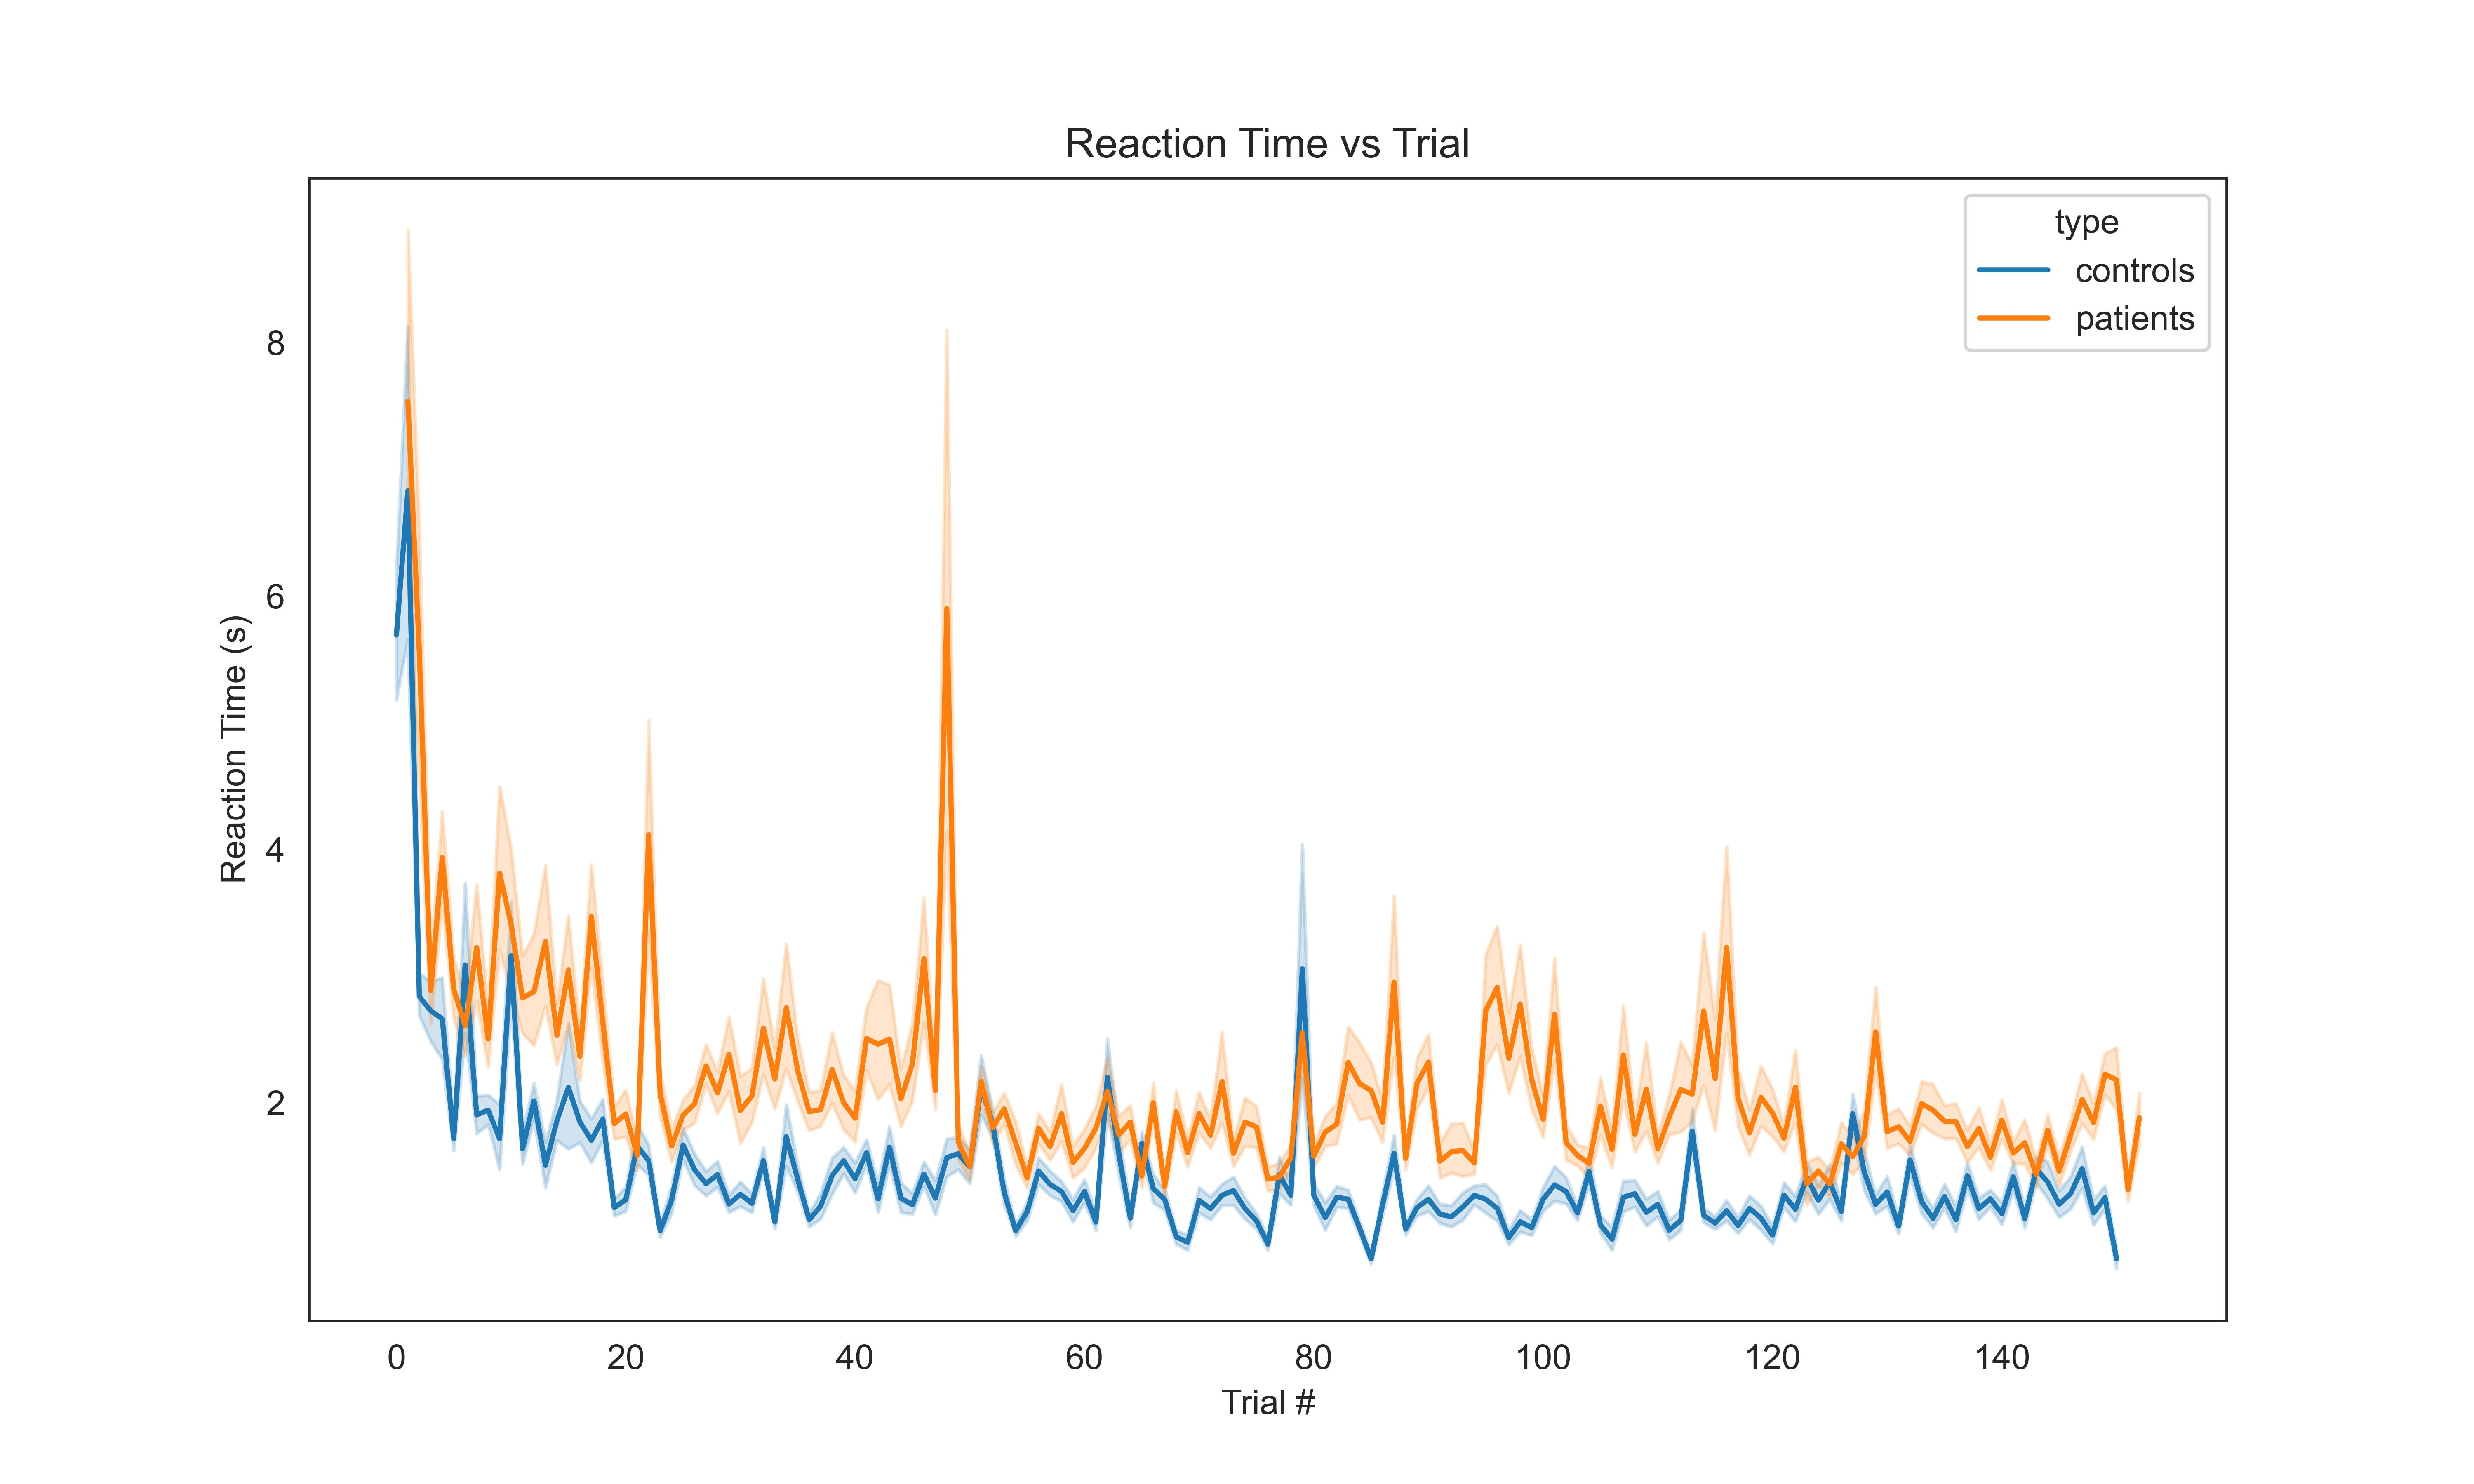
\includegraphics[width=15cm]{MainLayout/Images/chapter5/rt_clinical.jpg}
    \caption{Main Title for First Image \\ \small Subtitle for the first graphic.}
    \label{fig:rt_clinical}
\end{figure}

\begin{figure}[ht!]
    \centering
     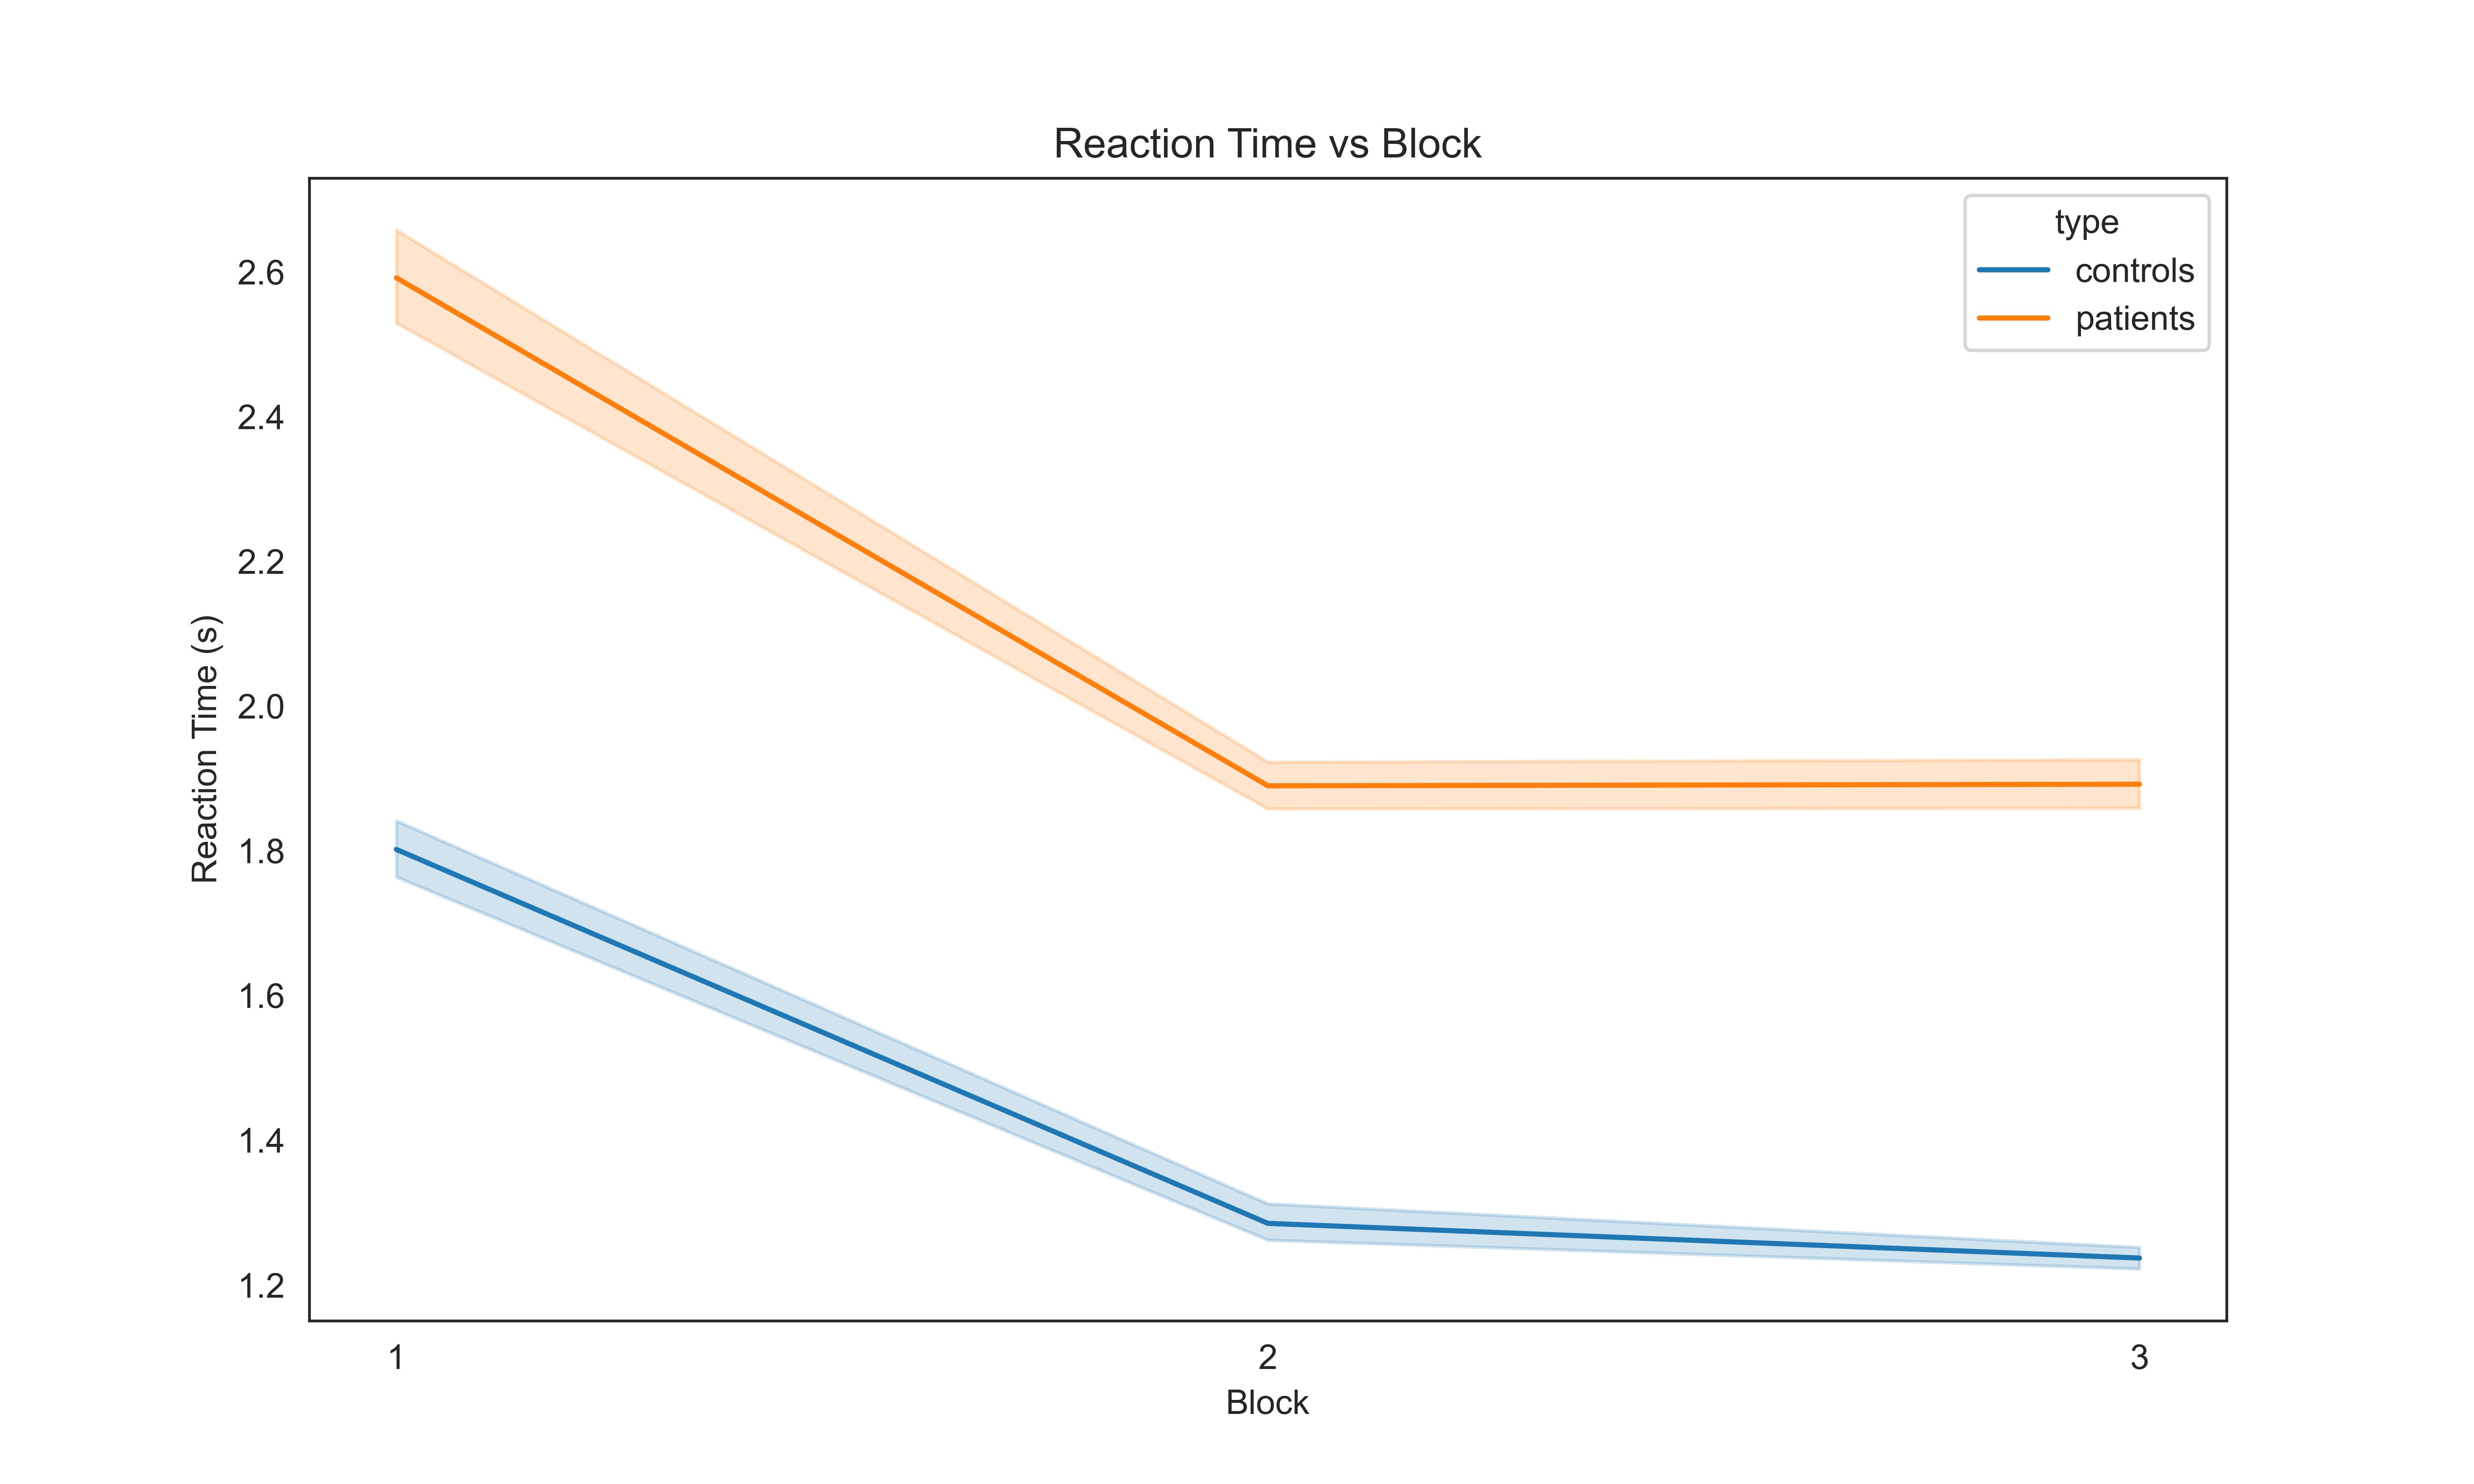
\includegraphics[width=15cm]{MainLayout/Images/chapter5/rt_block.jpg}
    \caption{Main Title for First Image \\ \small Subtitle for the first graphic.}
    \label{fig:rt_block}
\end{figure}

\begin{figure}[ht!]
    \centering
    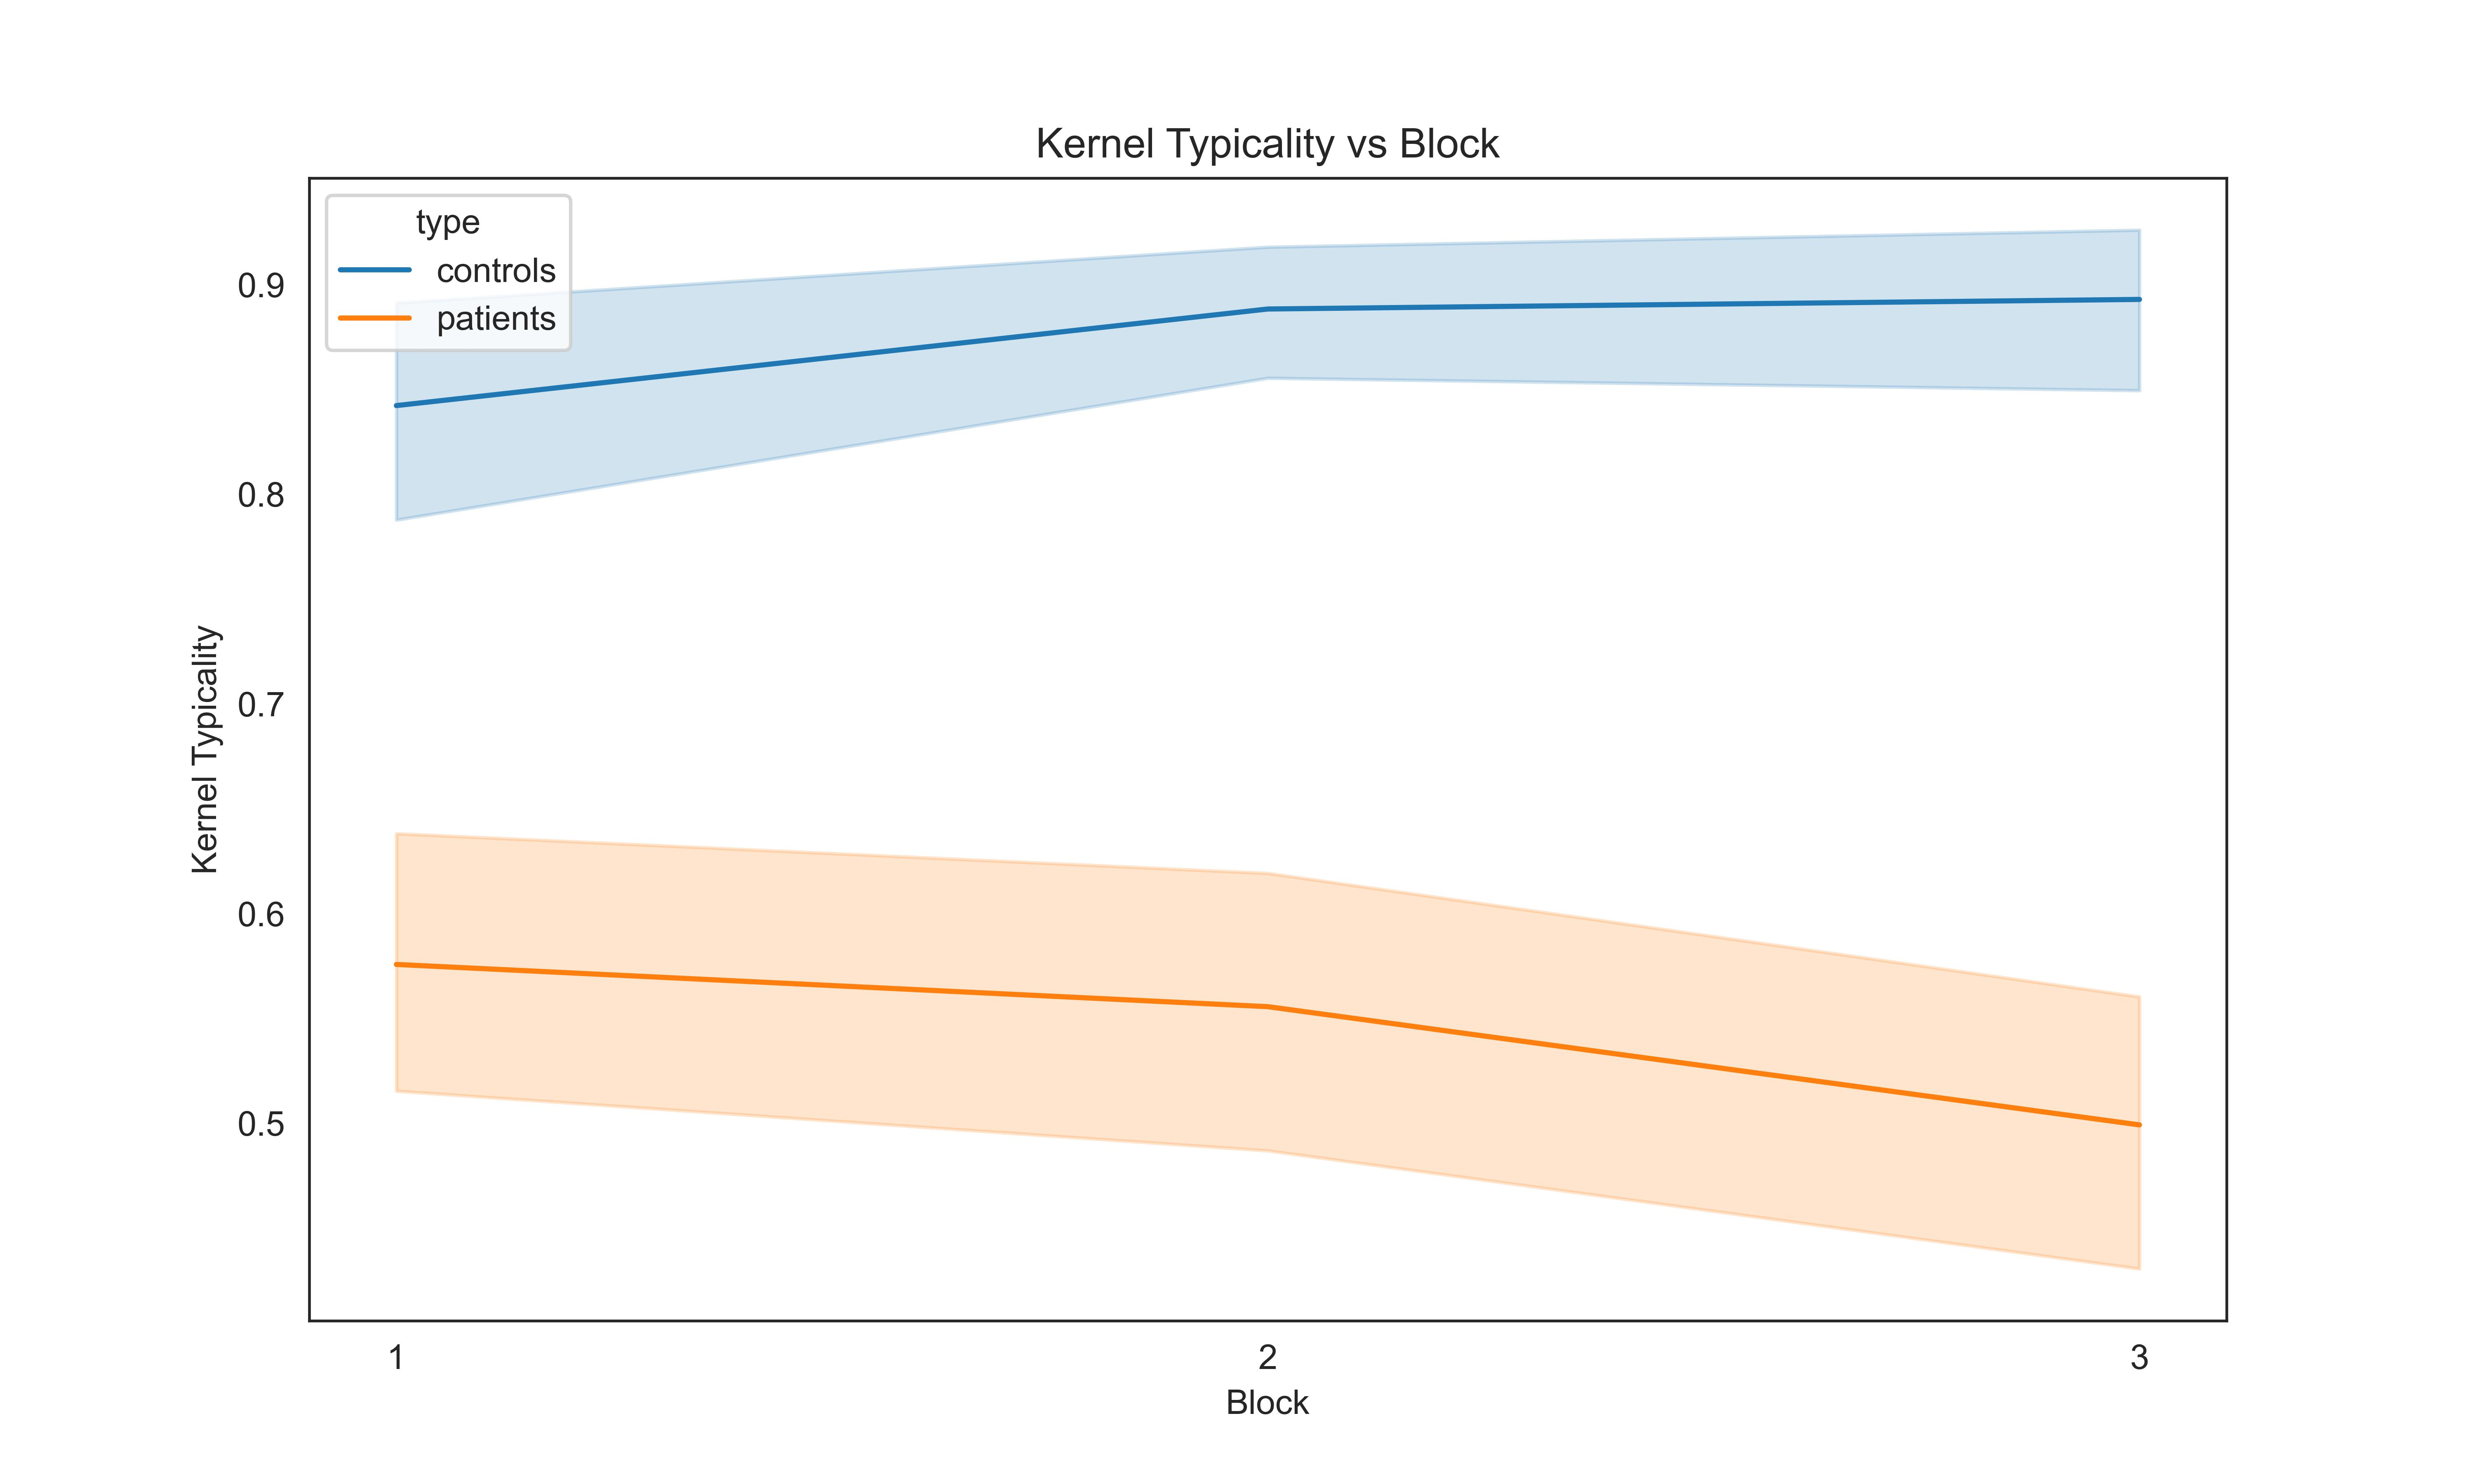
\includegraphics[width=15cm]{MainLayout/Images/chapter5/kernel_typicality_block.jpg}
    \caption{Main Title for First Image \\ \small Subtitle for the first graphic.}
    \label{fig:kernel_typicality_block}
\end{figure}

\subsection{Number of trials effects on kernel estimation}
The PALIN framework enables the simulation of a linear observer performing the same reverse correlation experiment as real participants, but with controlled parameters. We can simulate an experiment with limited trials (n=150) that observer has a known kernel(true) including 50 double-pass trials, repeated 1000 times to estimate the mental representation by two methods that already explained in chapter \ref{chap3} and evaluate the estimation error.

The figure \ref{fig:kernel_150} illustrates the relationship between the true internal noise and the kernel correlation (accuracy of mental representation estimation) for two kernel types: the weighted sum kernel (blue) and the GLM kernel (orange). The shaded areas represent the variability (confidence intervals) across 1000 simulations.



\begin{figure}[ht!]
    \centering
    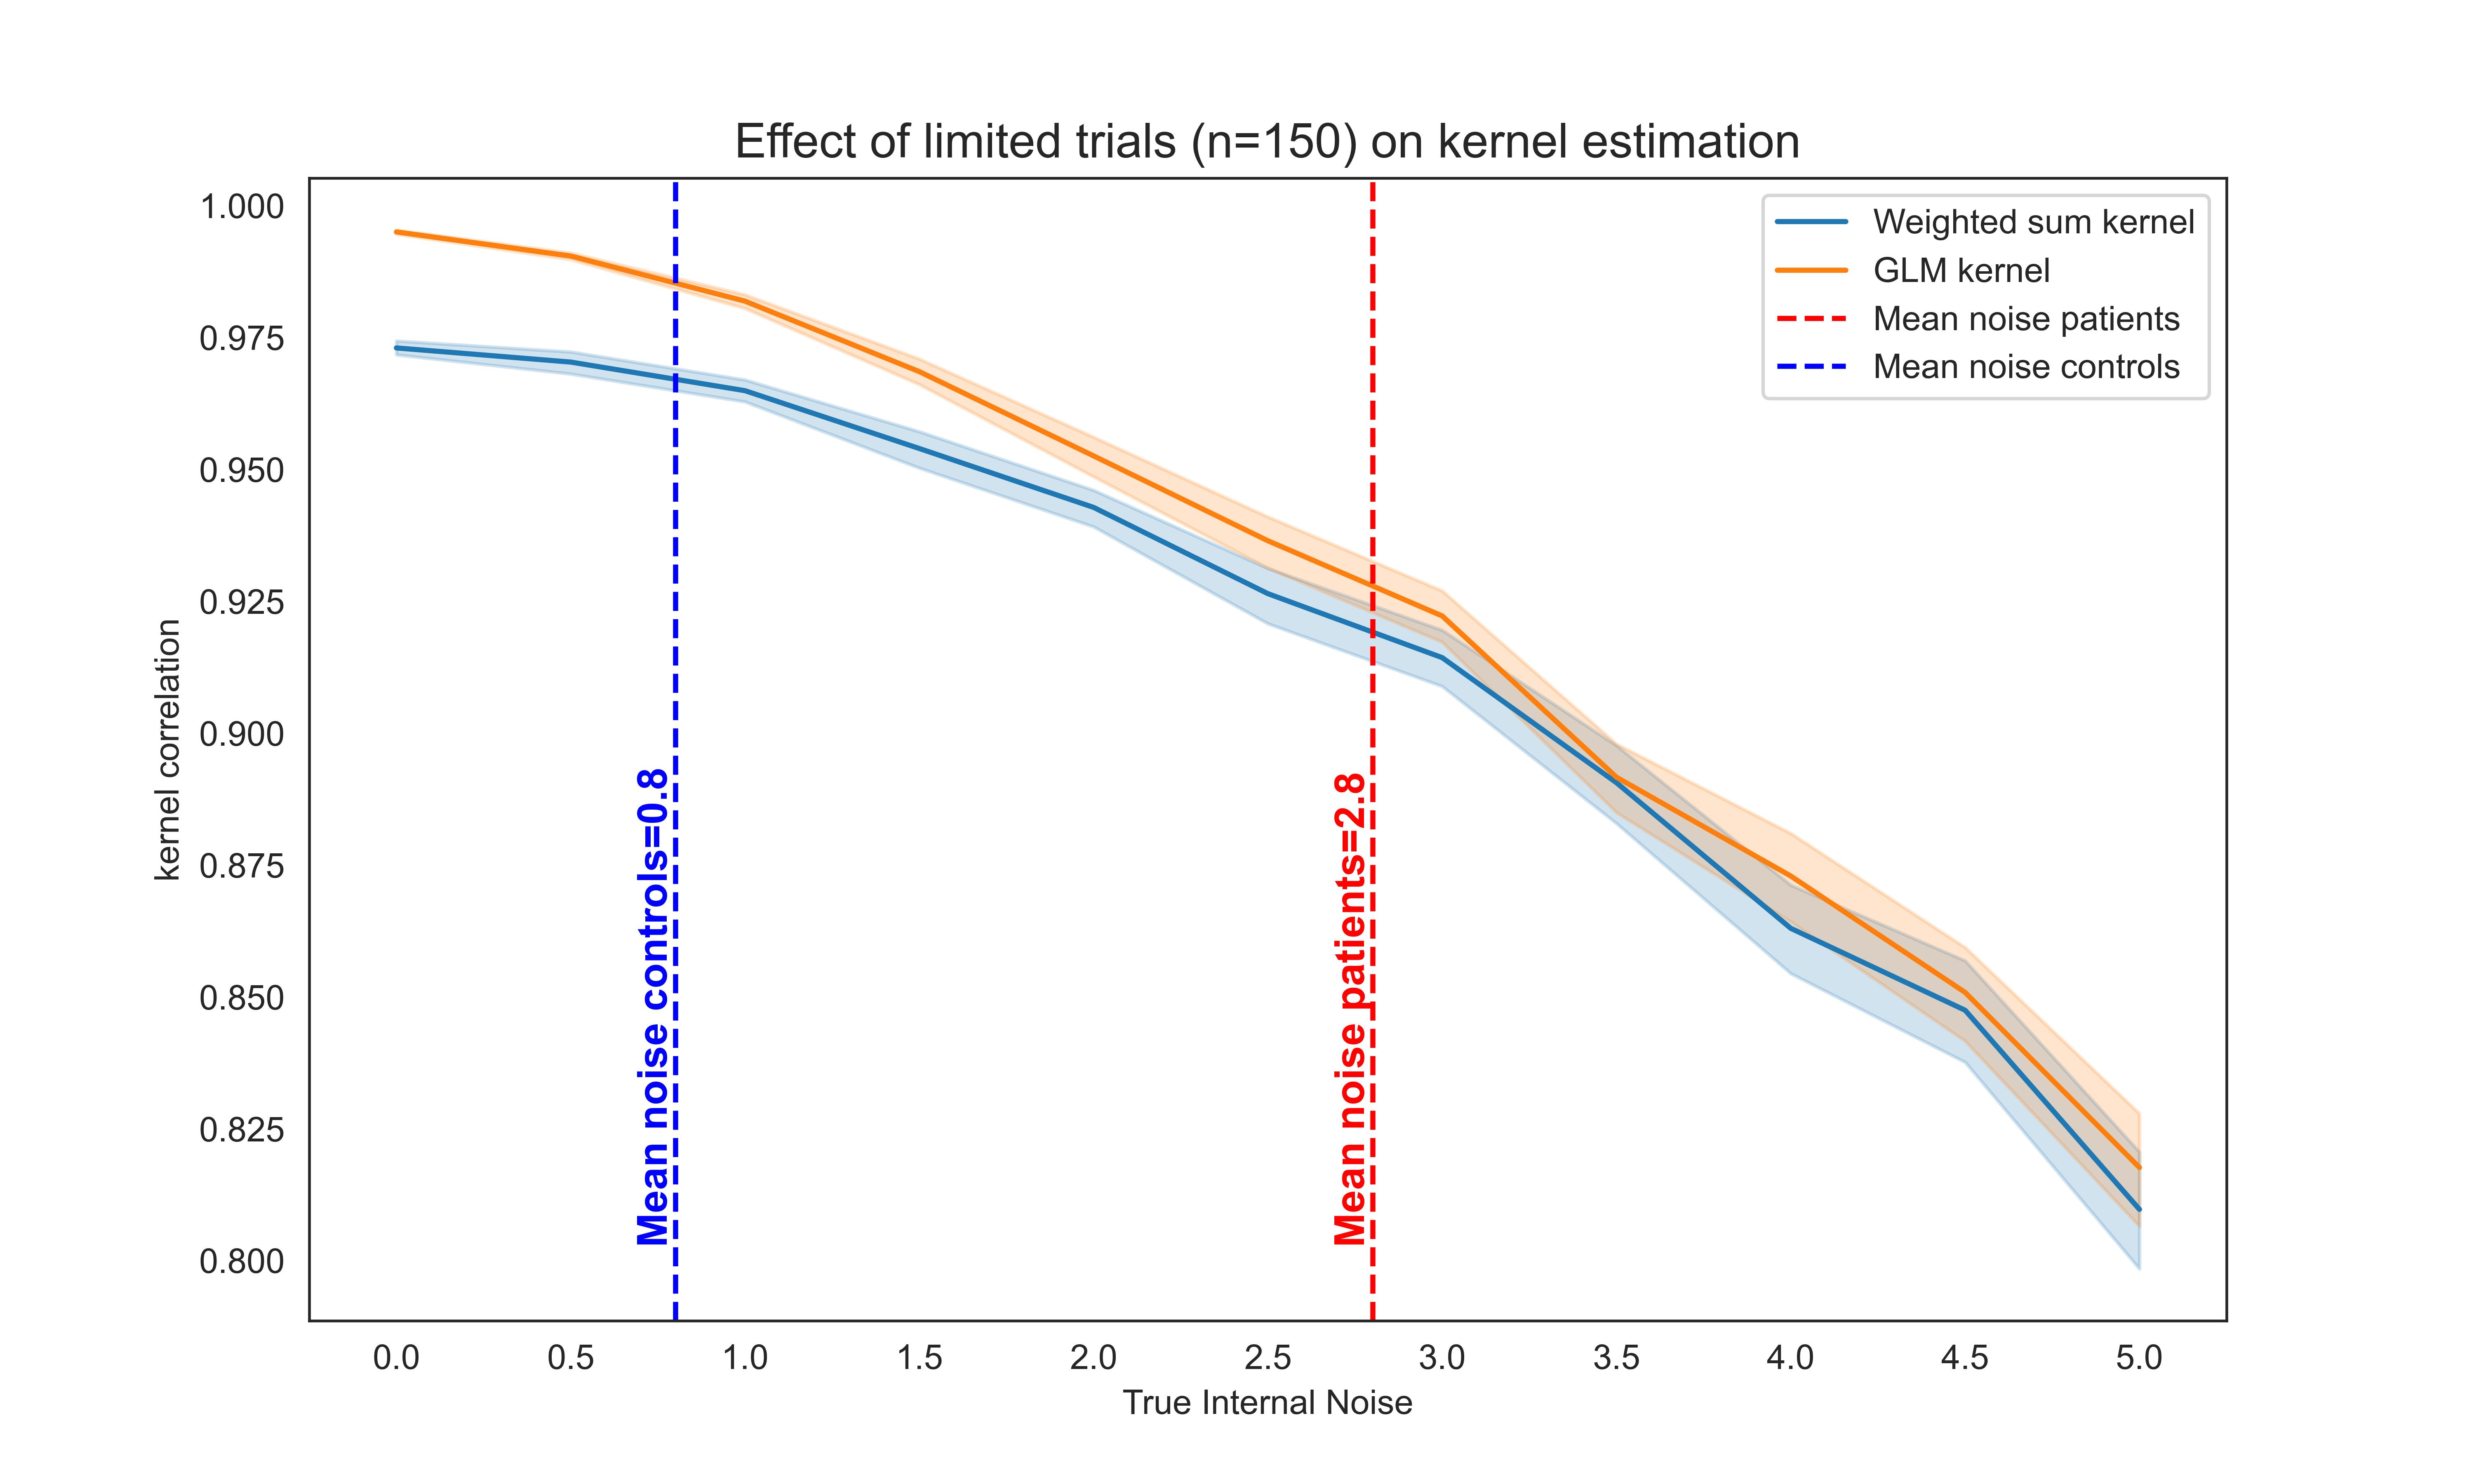
\includegraphics[width=15cm]{MainLayout/Images/chapter5/kernel_150.jpg}
    \caption{Main Title for First Image \\ \small Subtitle for the first graphic.}
    \label{fig:kernel_150}
\end{figure}
With only 50-150 trials, the double-pass method may not provide sufficient resolution to accurately estimate internal noise above a certain threshold (e.g., IN = 5).Monte Carlo simulations suggest that for values of IN > 5, increasing the number of trials (e.g., to 1000 or more) is necessary to get stable estimates.
In stroke patients, where trials are often limited due to fatigue or cognitive impairment, the estimation method might not capture their true perceptual variability.
When the number of double-pass trials is small (e.g., 50-150 trials), the variance in internal noise estimation increases.
Confidence intervals widen significantly, making it difficult to differentiate noise values above a certain threshold.
Empirical simulations show that IN estimates tend to be overestimated for values <6 and underestimated for values >6.
Another major methodological limitation arises from trial count restrictions. Estimating internal noise requires a substantial number of repeated trials for statistical reliability, yet in clinical populations such as stroke patients, lengthy experimental sessions are not feasible due to fatigue and attentional constraints. As a result, the limited number of trials introduces a high degree of variability in the estimated internal noise, making the measurement less reliable. Additionally, the method does not account for response perseveration, a phenomenon frequently observed in stroke patients with right-hemisphere damage. Perseveration can artificially inflate estimates of internal noise because the model assumes that repeated trials are independent, whereas in reality, some patients persistently select the same response across multiple trials regardless of the presented stimulus. This means that some patients may appear to have high internal noise simply due to habitual responding rather than perceptual instability.



\subsection{Number of trials effects on internal noise estimation}

Beyond these theoretical and methodological concerns, practical limitations also affect the applicability of Monte Carlo simulations in clinical settings. The estimation process requires large-scale simulations across a wide range of internal noise and bias values, making the approach computationally intensive. Running thousands of simulated trials to obtain stable estimates is feasible for offline analysis but becomes impractical for real-time clinical assessments where fast, efficient estimation methods are needed. Additionally, the method assumes that patient behavior conforms to the SDT framework, but in reality, some stroke survivors may demonstrate idiosyncratic decision-making strategies that fall outside of the model’s assumptions. This means that the estimated internal noise may not always reflect true perceptual variability but instead capture artifacts introduced by strategy shifts, attentional fluctuations, or cognitive rigidity.

\begin{figure}[ht!]
    \centering
    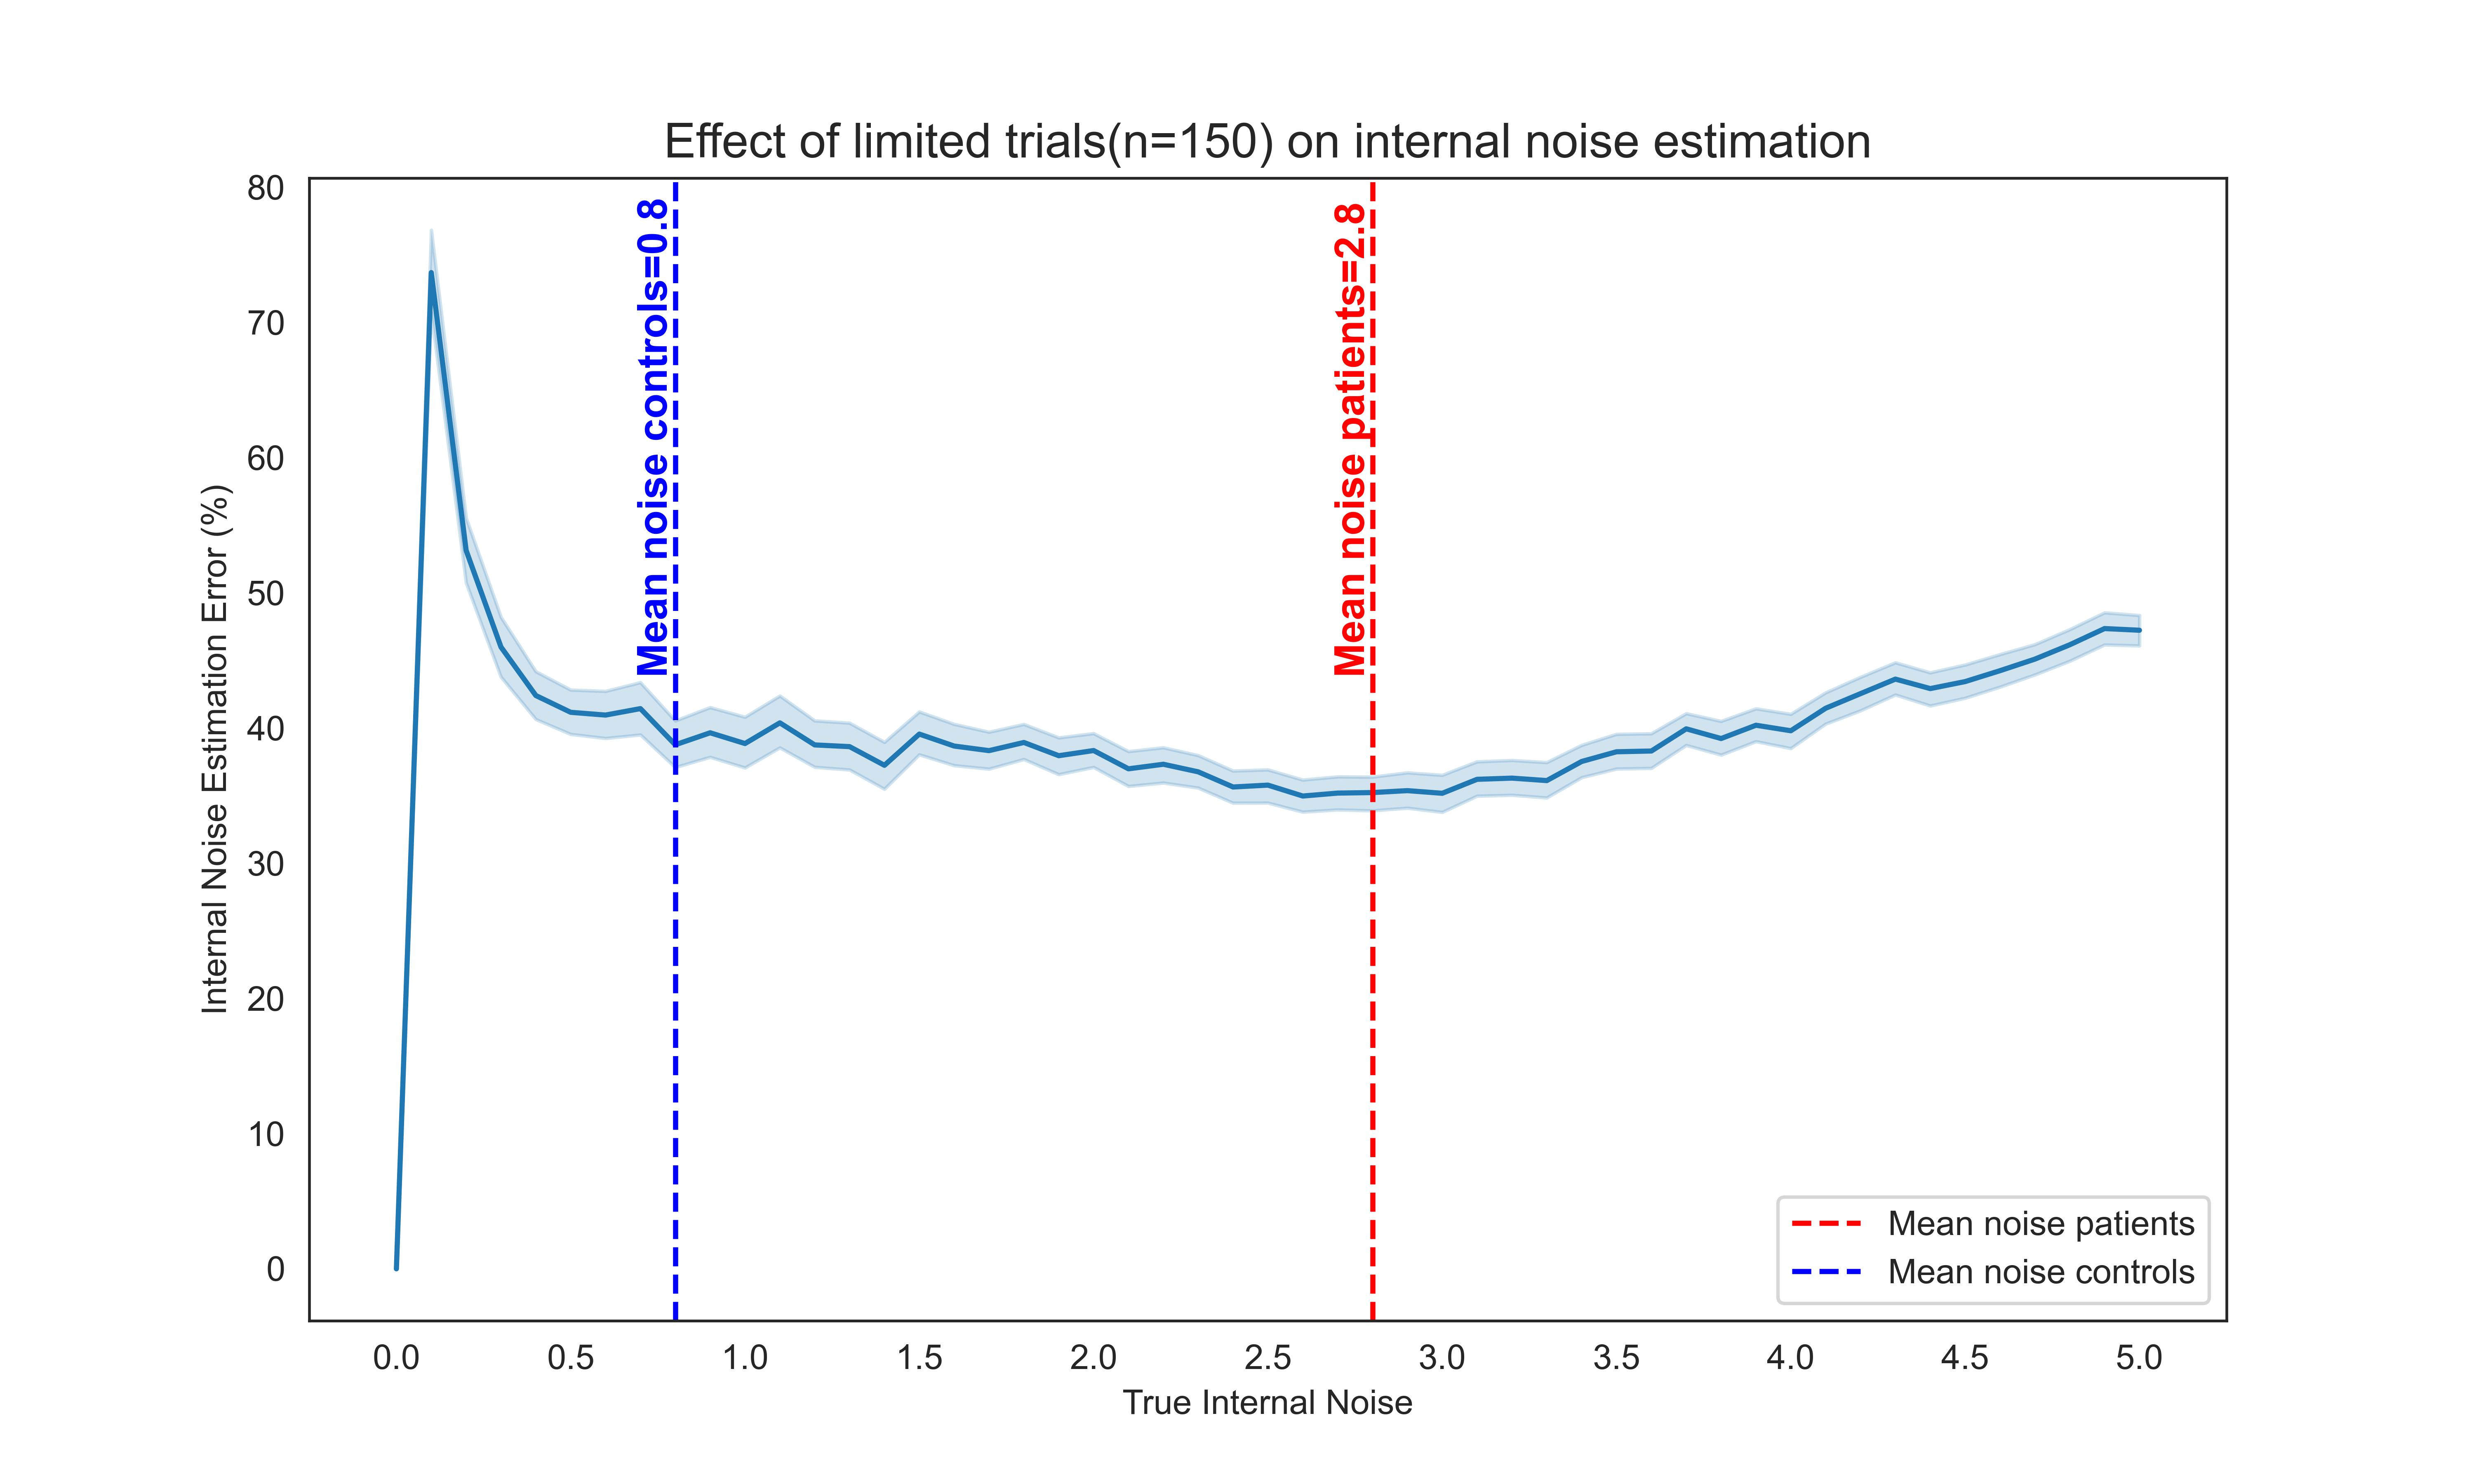
\includegraphics[width=15cm]{MainLayout/Images/chapter5/noise_150.jpg}
    \caption{Main Title for First Image \\ \small Subtitle for the first graphic.}
    \label{fig:noise_150}
\end{figure}

\begin{figure}[ht!]
    \centering
    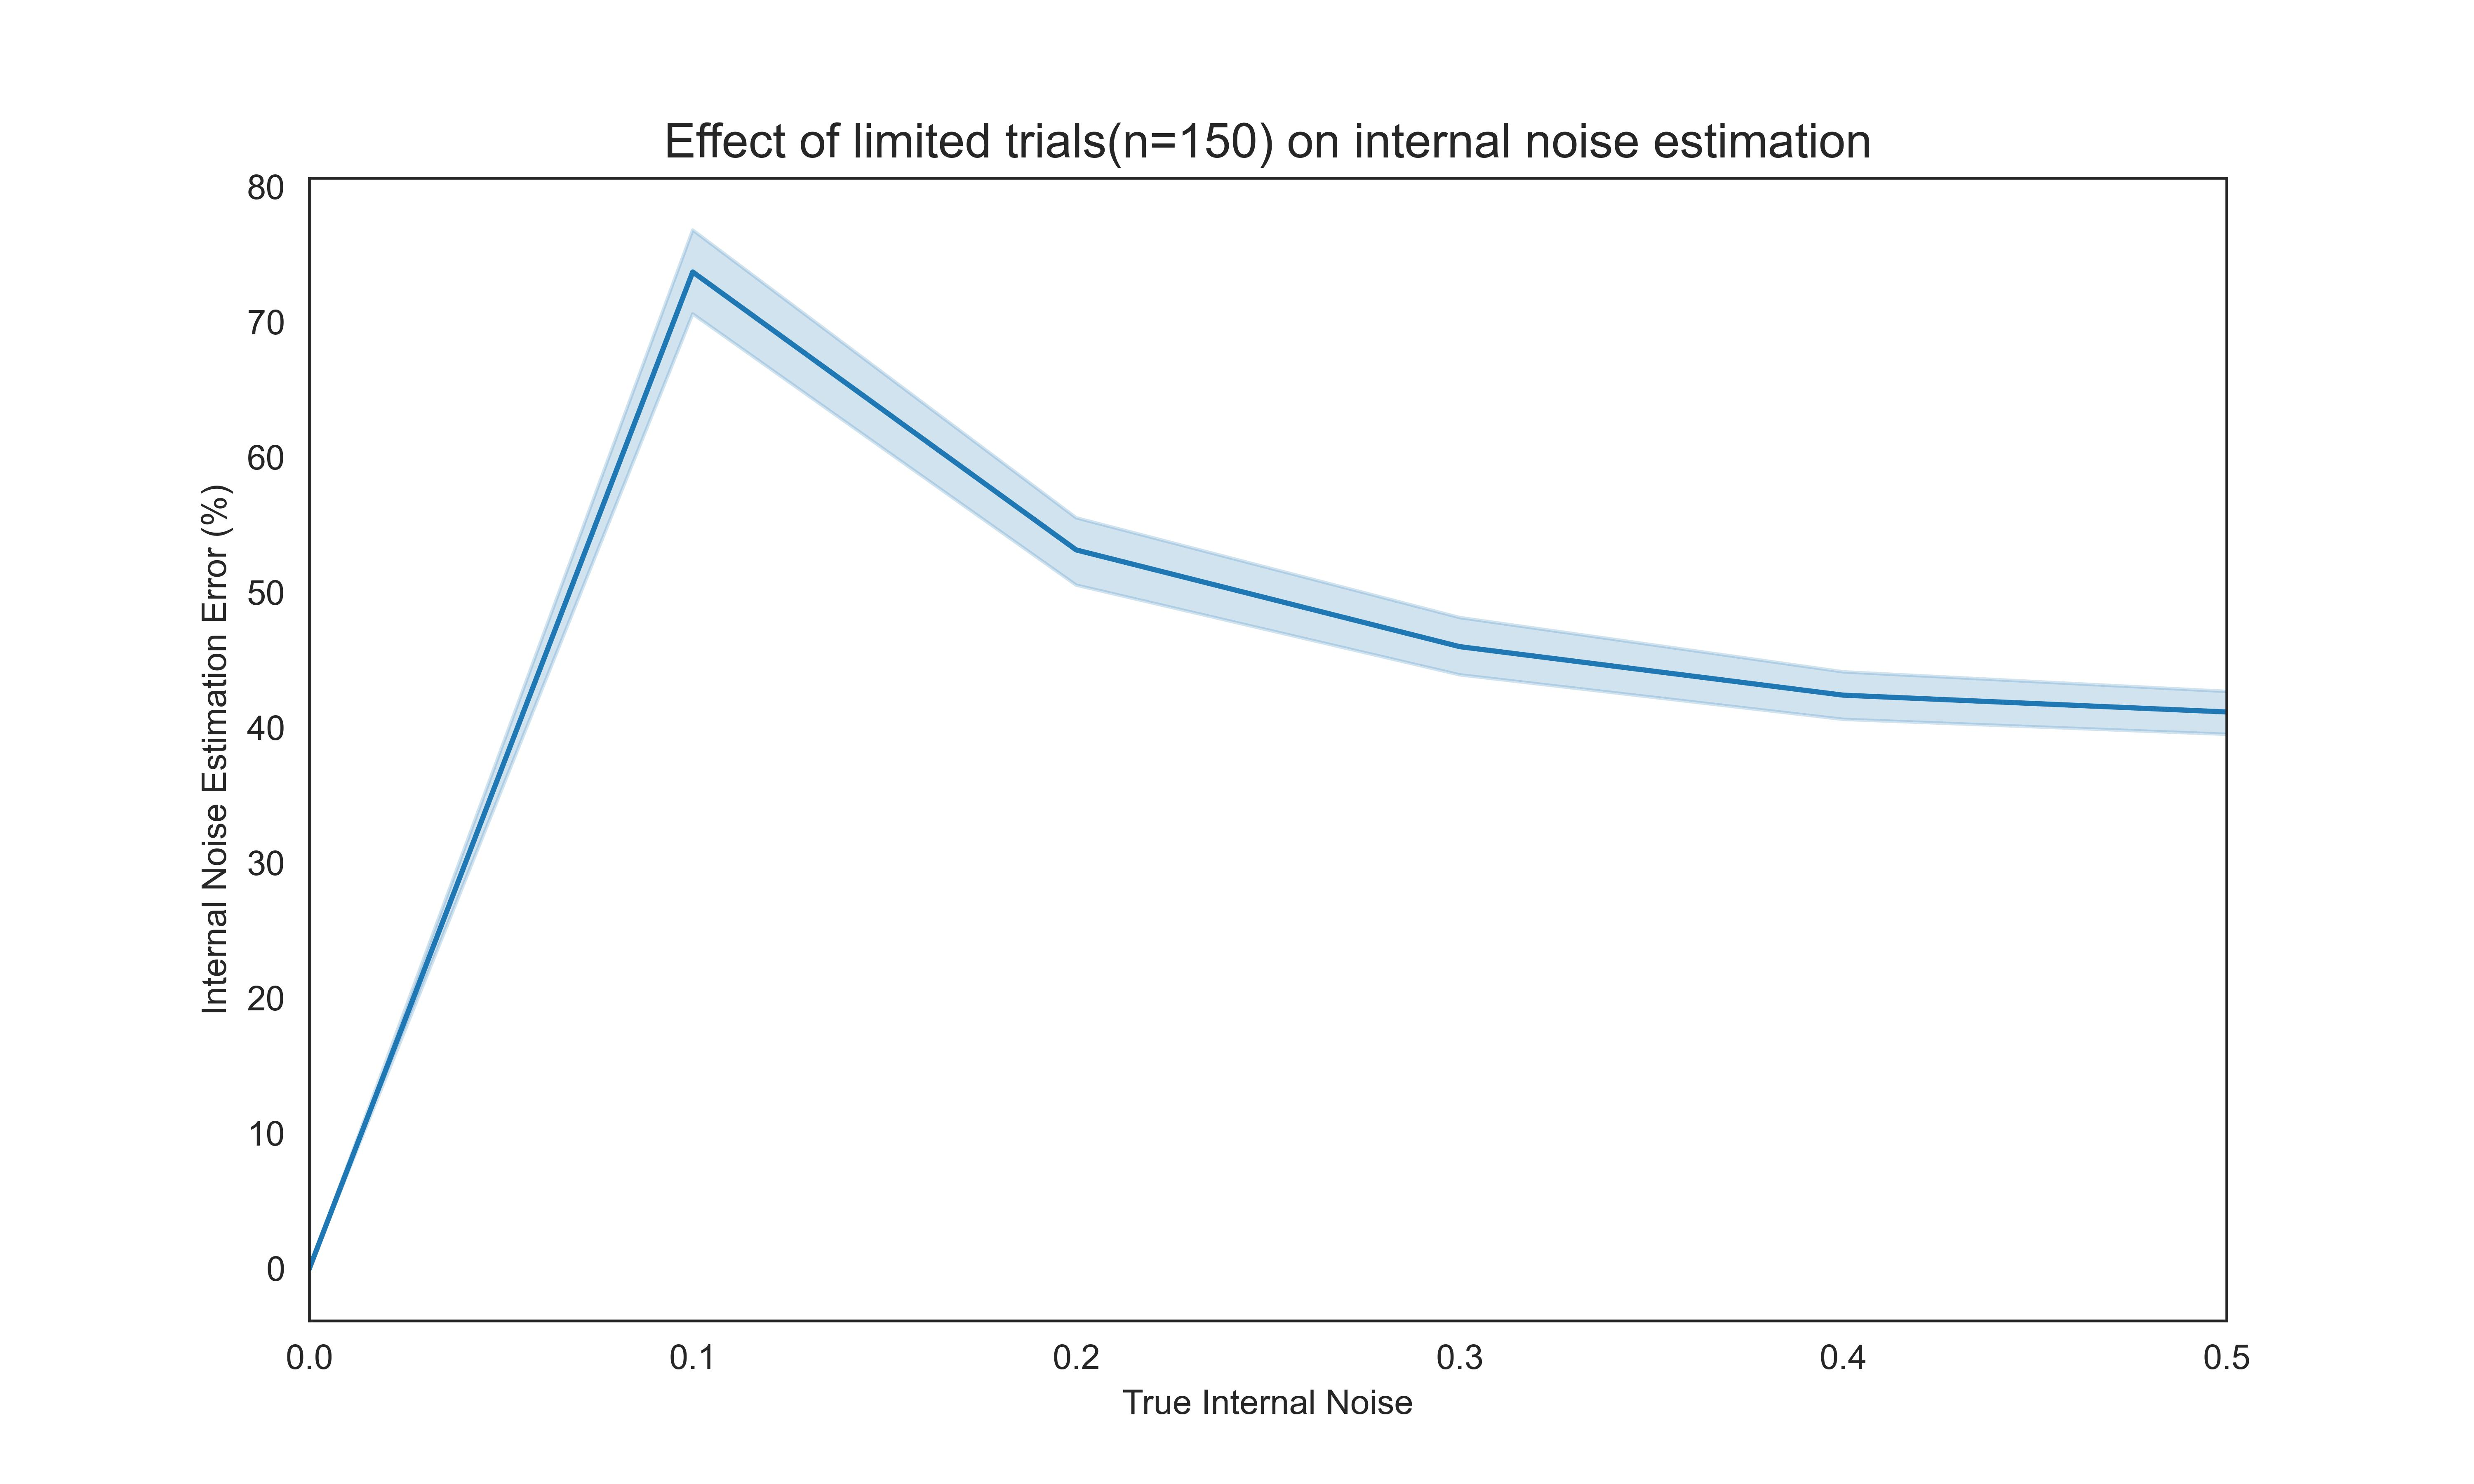
\includegraphics[width=15cm]{MainLayout/Images/chapter5/noise_150_0to05.jpg}
    \caption{Main Title for First Image \\ \small Subtitle for the first graphic.}
    \label{fig:noise_150_0to05}
\end{figure}
\section {Perseveration} 

\subsection {Perseveration a consequence of stroke} 
%It is possible that their excessive responses do not align with the average pathological profiles, leading to misclassification. 

By examining responses closely, we observe that some patients consistently chose the same stimulus across multiple trials without variation. As previously discussed, this behavior may result from attentional challenges following right-hemisphere stroke or symptoms of spatial neglect. This pattern has also been notably observed during speech and language therapy (SLT) sessions by therapists, further highlighting its clinical relevance. 

From the perspective of the linear observer model and signal detection theory, participants exhibiting perseverative behavior no longer rely on their decision model to guide their responses. Instead of making choices based on their mental representation, they disengage from actively applying it to the stimuli. As a result, their responses become detached from stimulus evaluation, suggesting a lack of attentional control in determining which stimulus should be chosen.

Several established tasks exist for quantifying perseveration, such as Object Alternation (OA) \cite{freedman_orbitofrontal_1998} and the Wisconsin Card Sorting Test (WCST) \cite{abbruzzese_performance_1996}, which are widely used in assessing cognitive rigidity in conditions like aphasia and schizophrenia. These tasks measure executive function impairments, including difficulty in adapting to rule changes and excessive response repetition. However, despite their use in broader neuropsychological research, they have not been systematically applied to evaluate prosody perception deficits after stroke. Investigating whether similar mechanisms of perseveration extend to prosodic processing could provide new insights into the relationship between executive function deficits and speech impairments in stroke patients.

\begin{figure}[ht!]
    \centering
    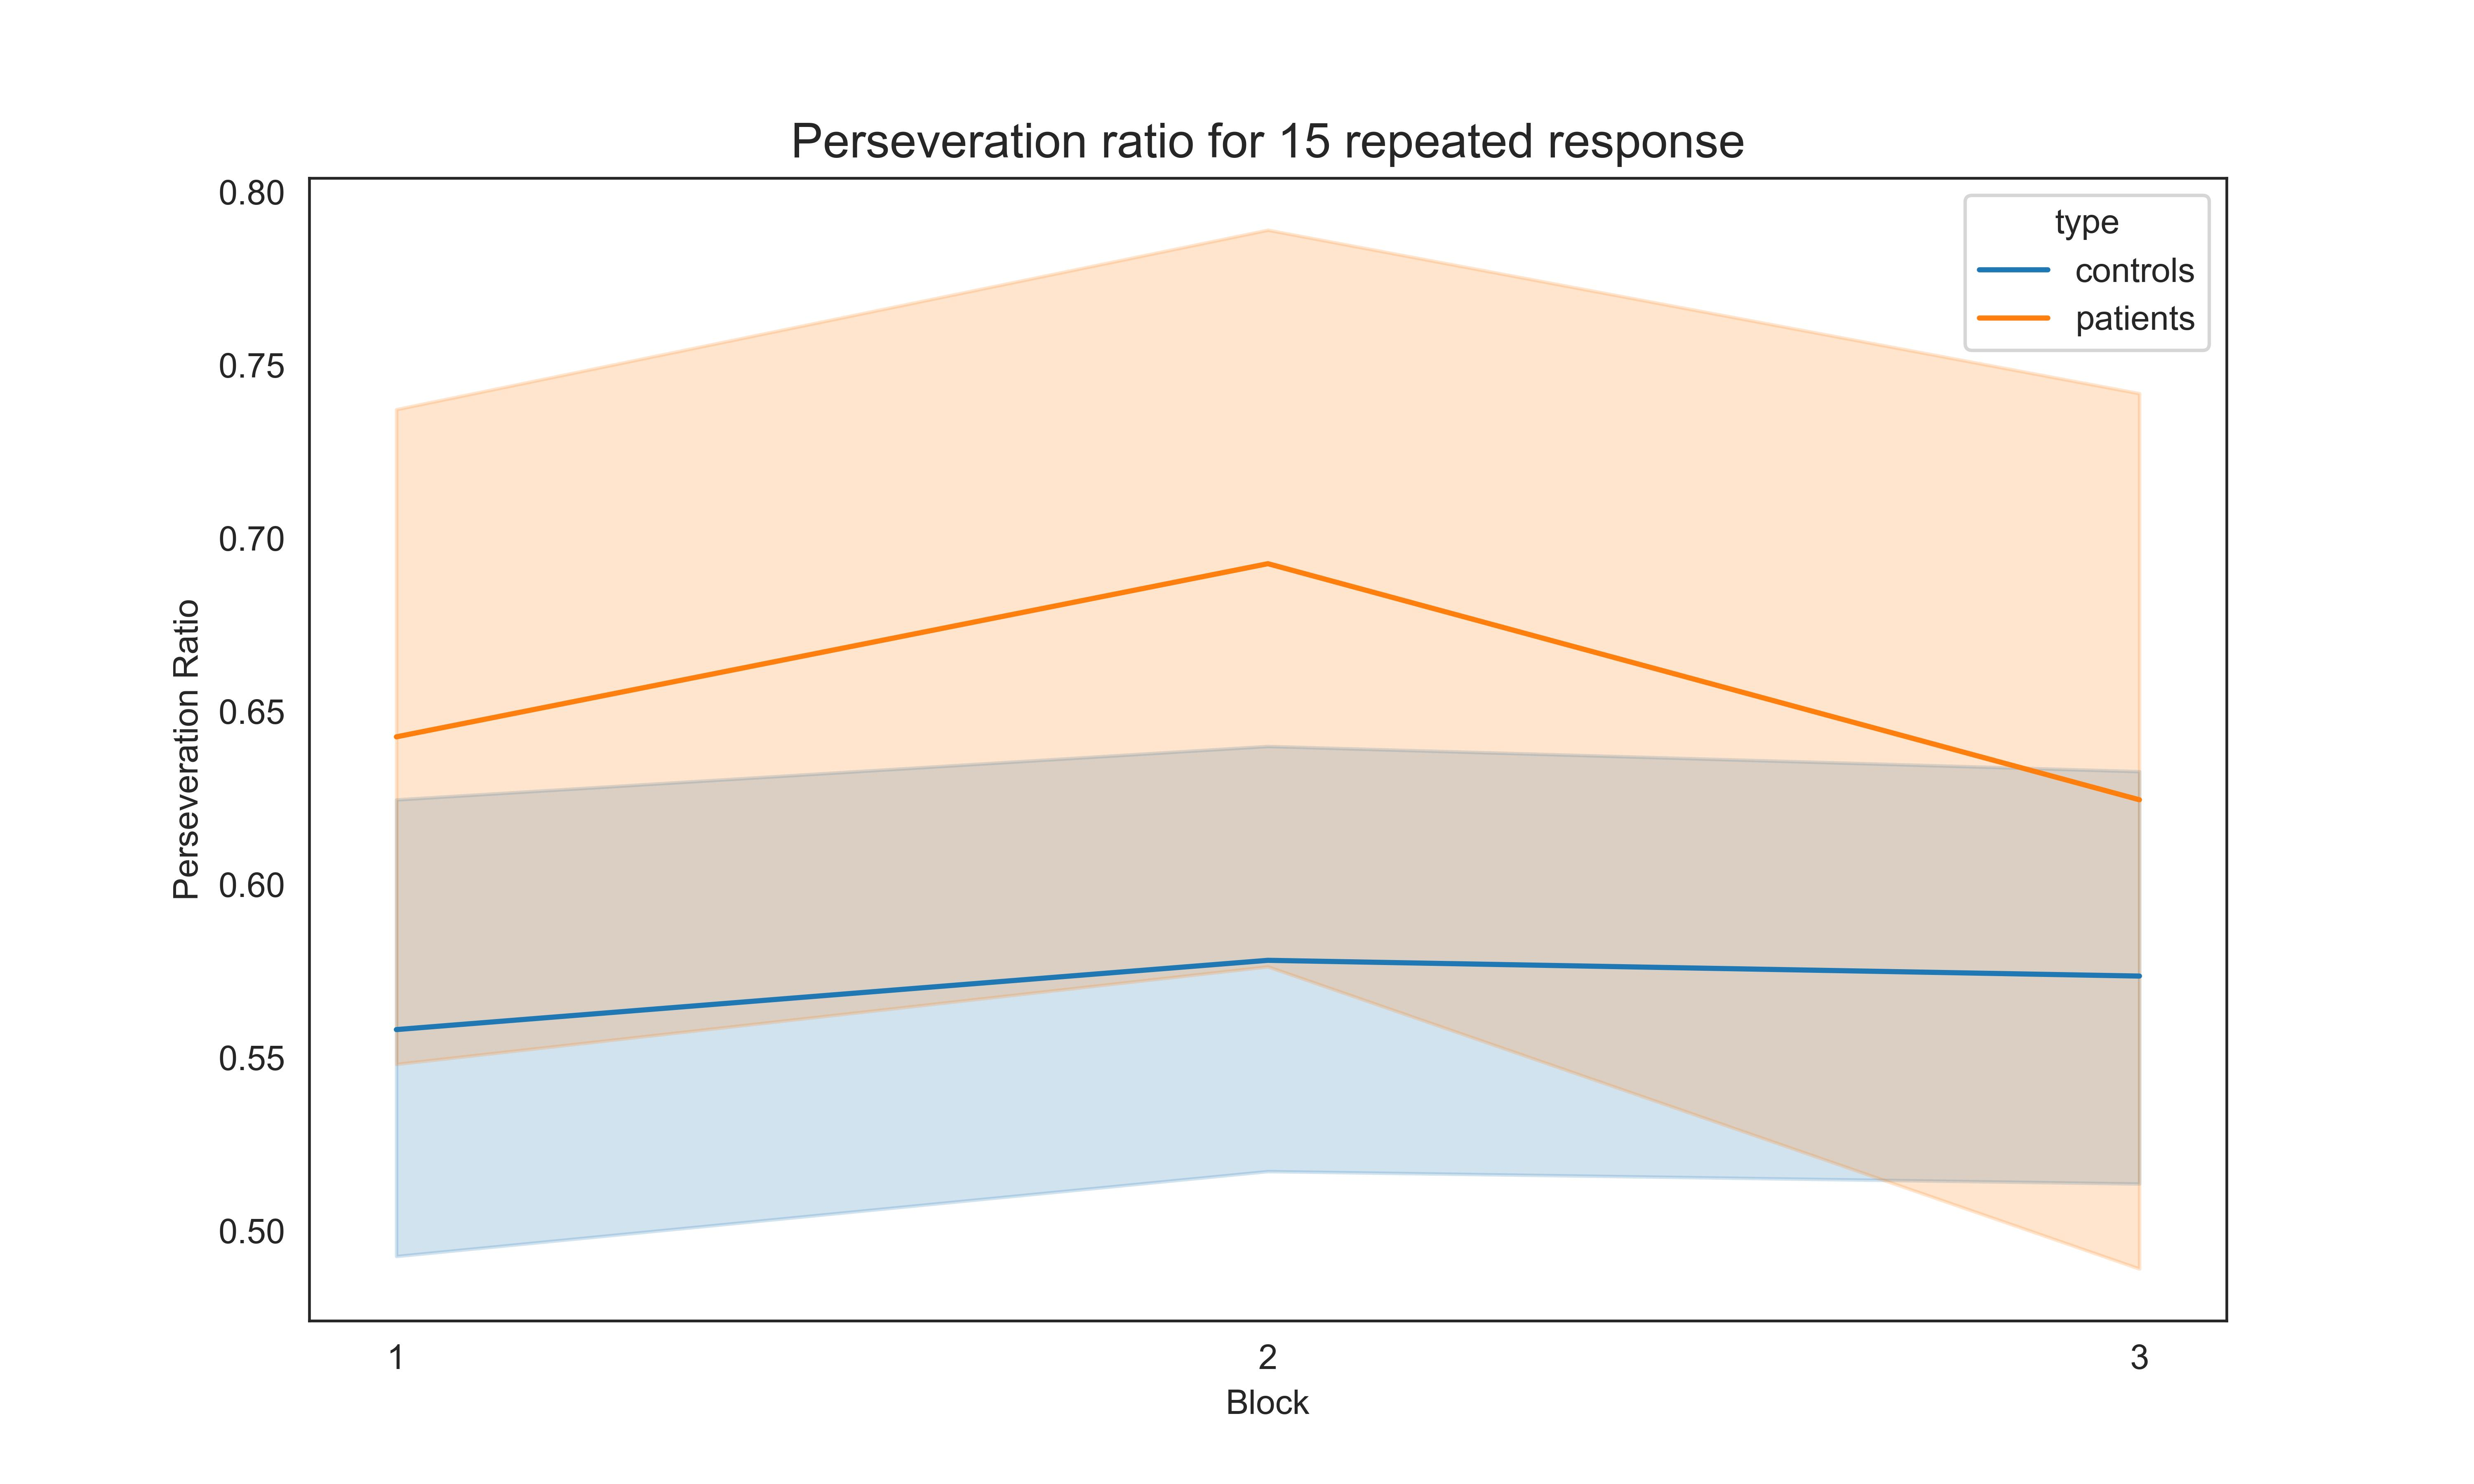
\includegraphics[width=15cm]{MainLayout/Images/chapter5/perseveration_block.jpg}
    \caption{Main Title for First Image \\ \small Subtitle for the first graphic.}
    \label{fig:perseveration_block}
\end{figure}
\subsection{Perseveration effects on kernel estimation}
\begin{figure}[ht!]
    \centering
    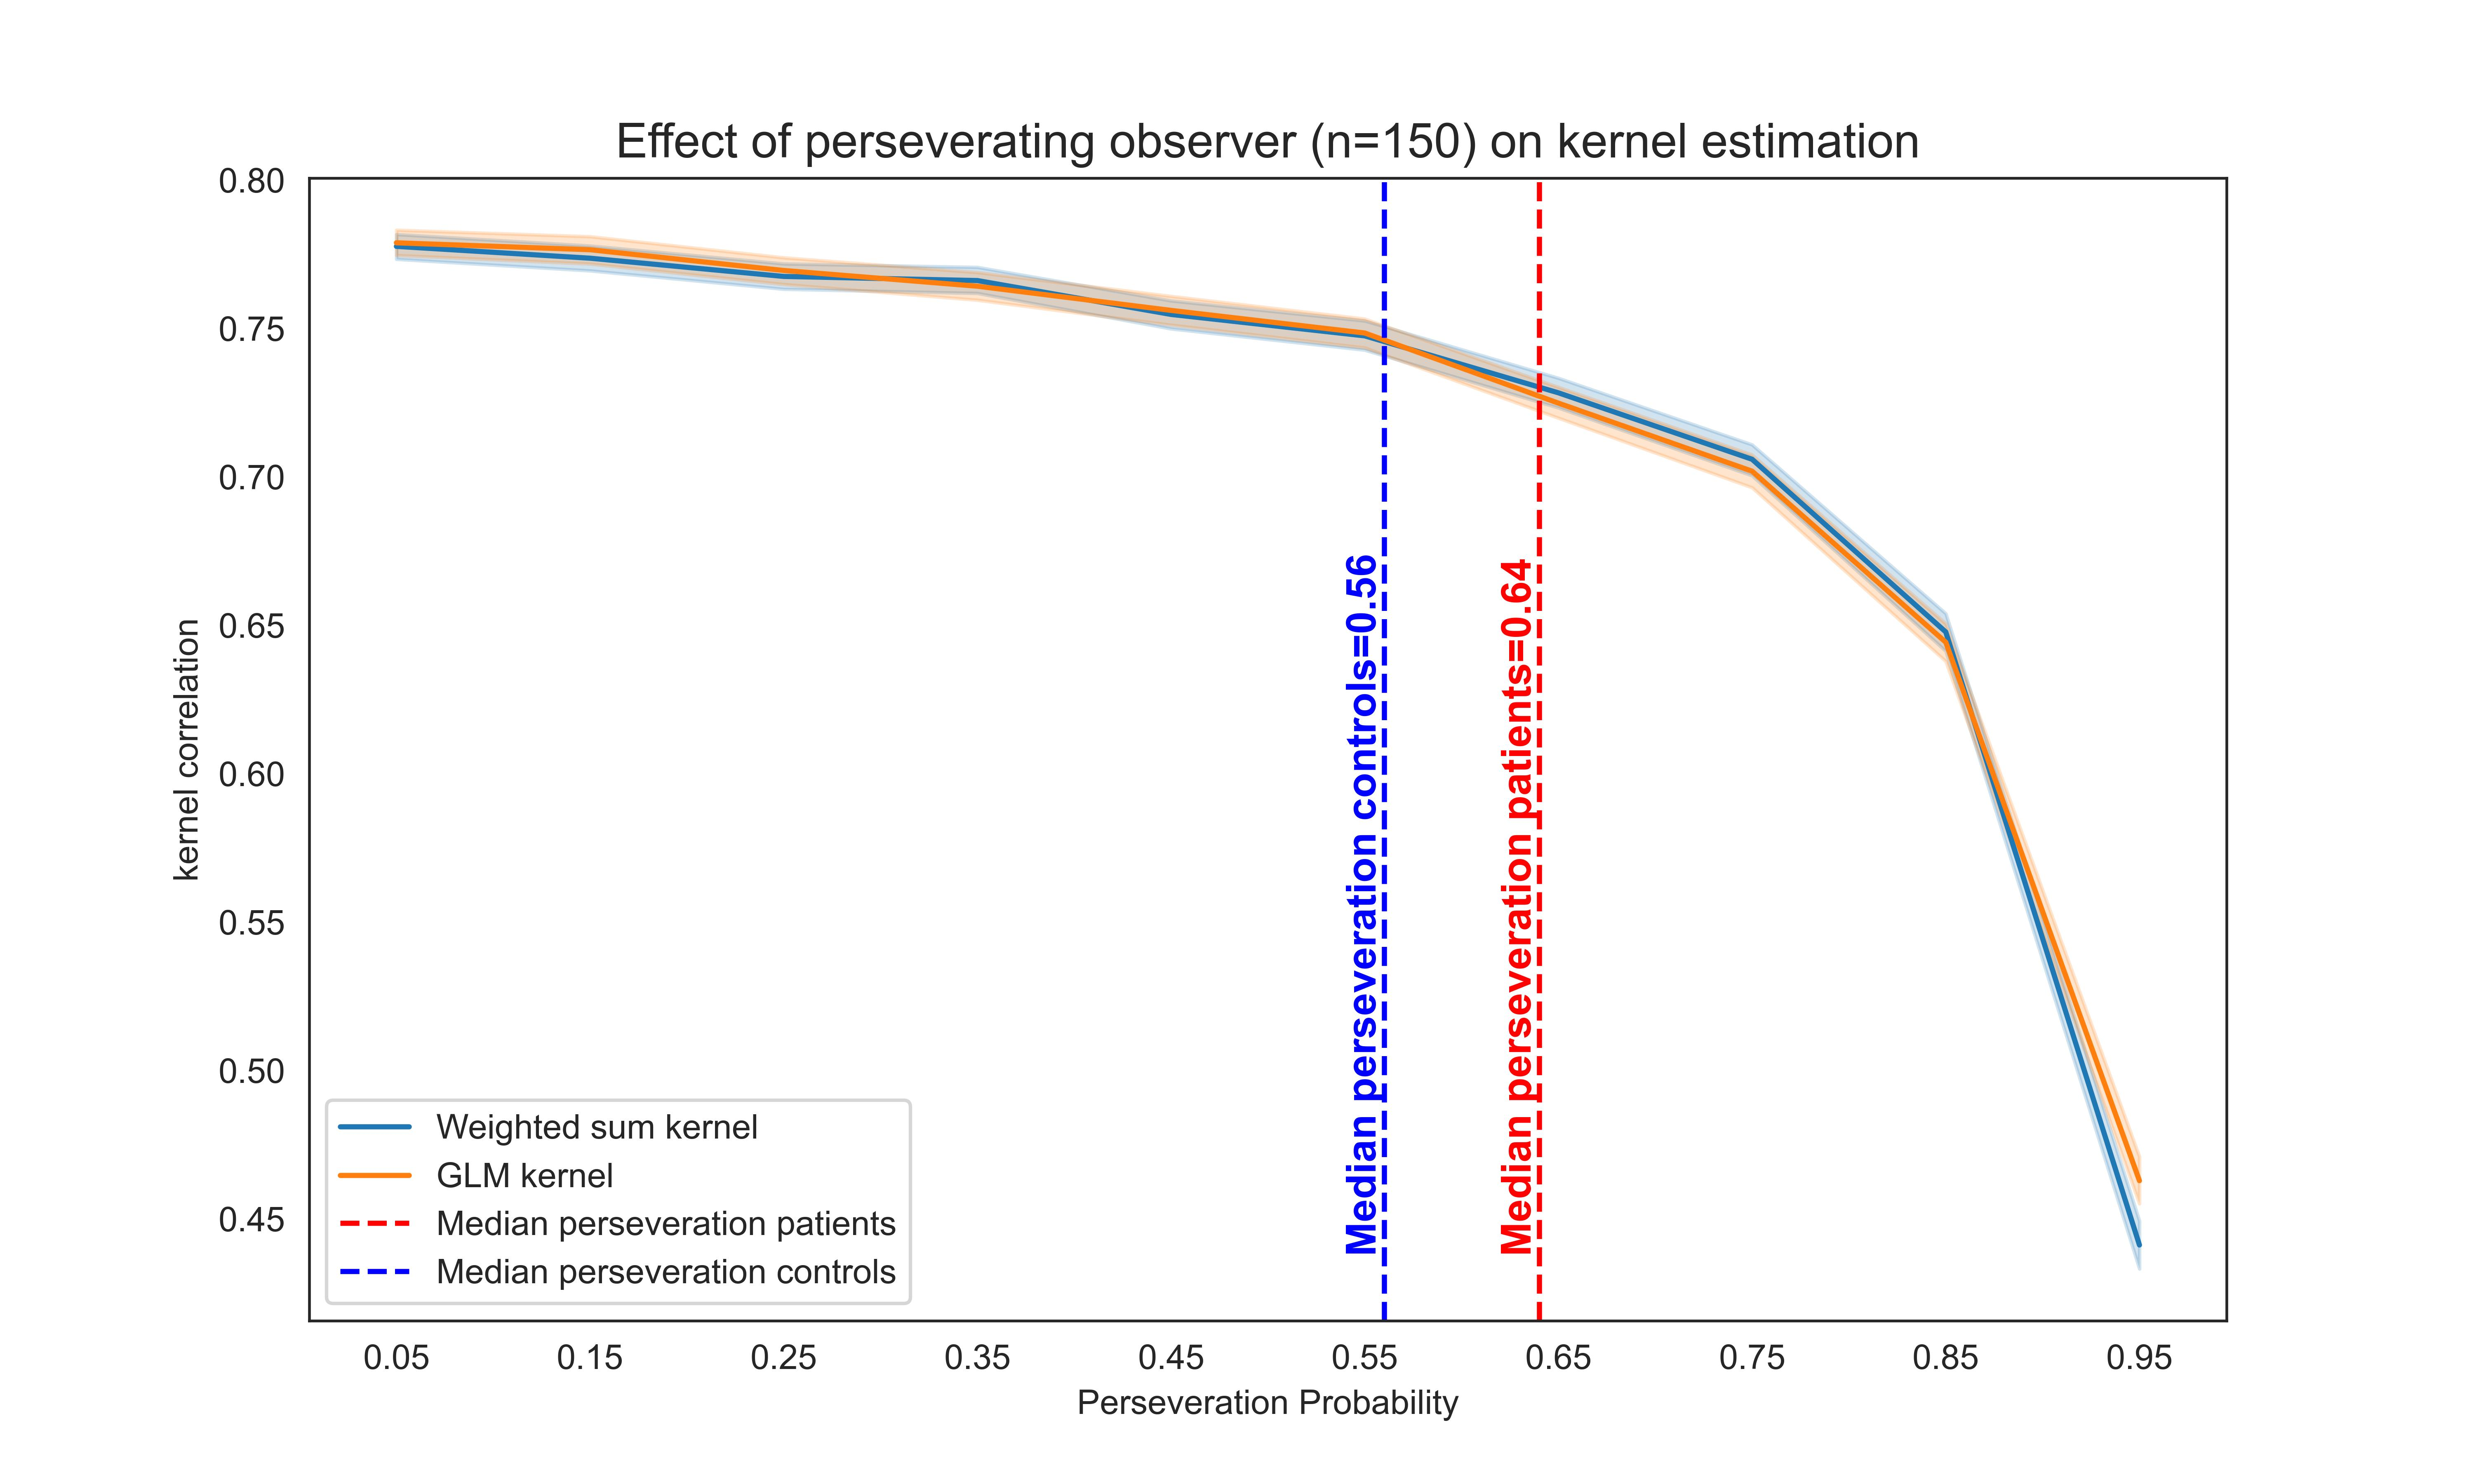
\includegraphics[width=15cm]{MainLayout/Images/chapter5/kernel_perseverating_observer.jpg}
    \caption{Main Title for First Image \\ \small Subtitle for the first graphic.}
    \label{fig:kernel_perseverating_observer}
\end{figure}
\subsection{Perseveration effects on internal noise estimation}

\begin{figure}[ht!]
    \centering
    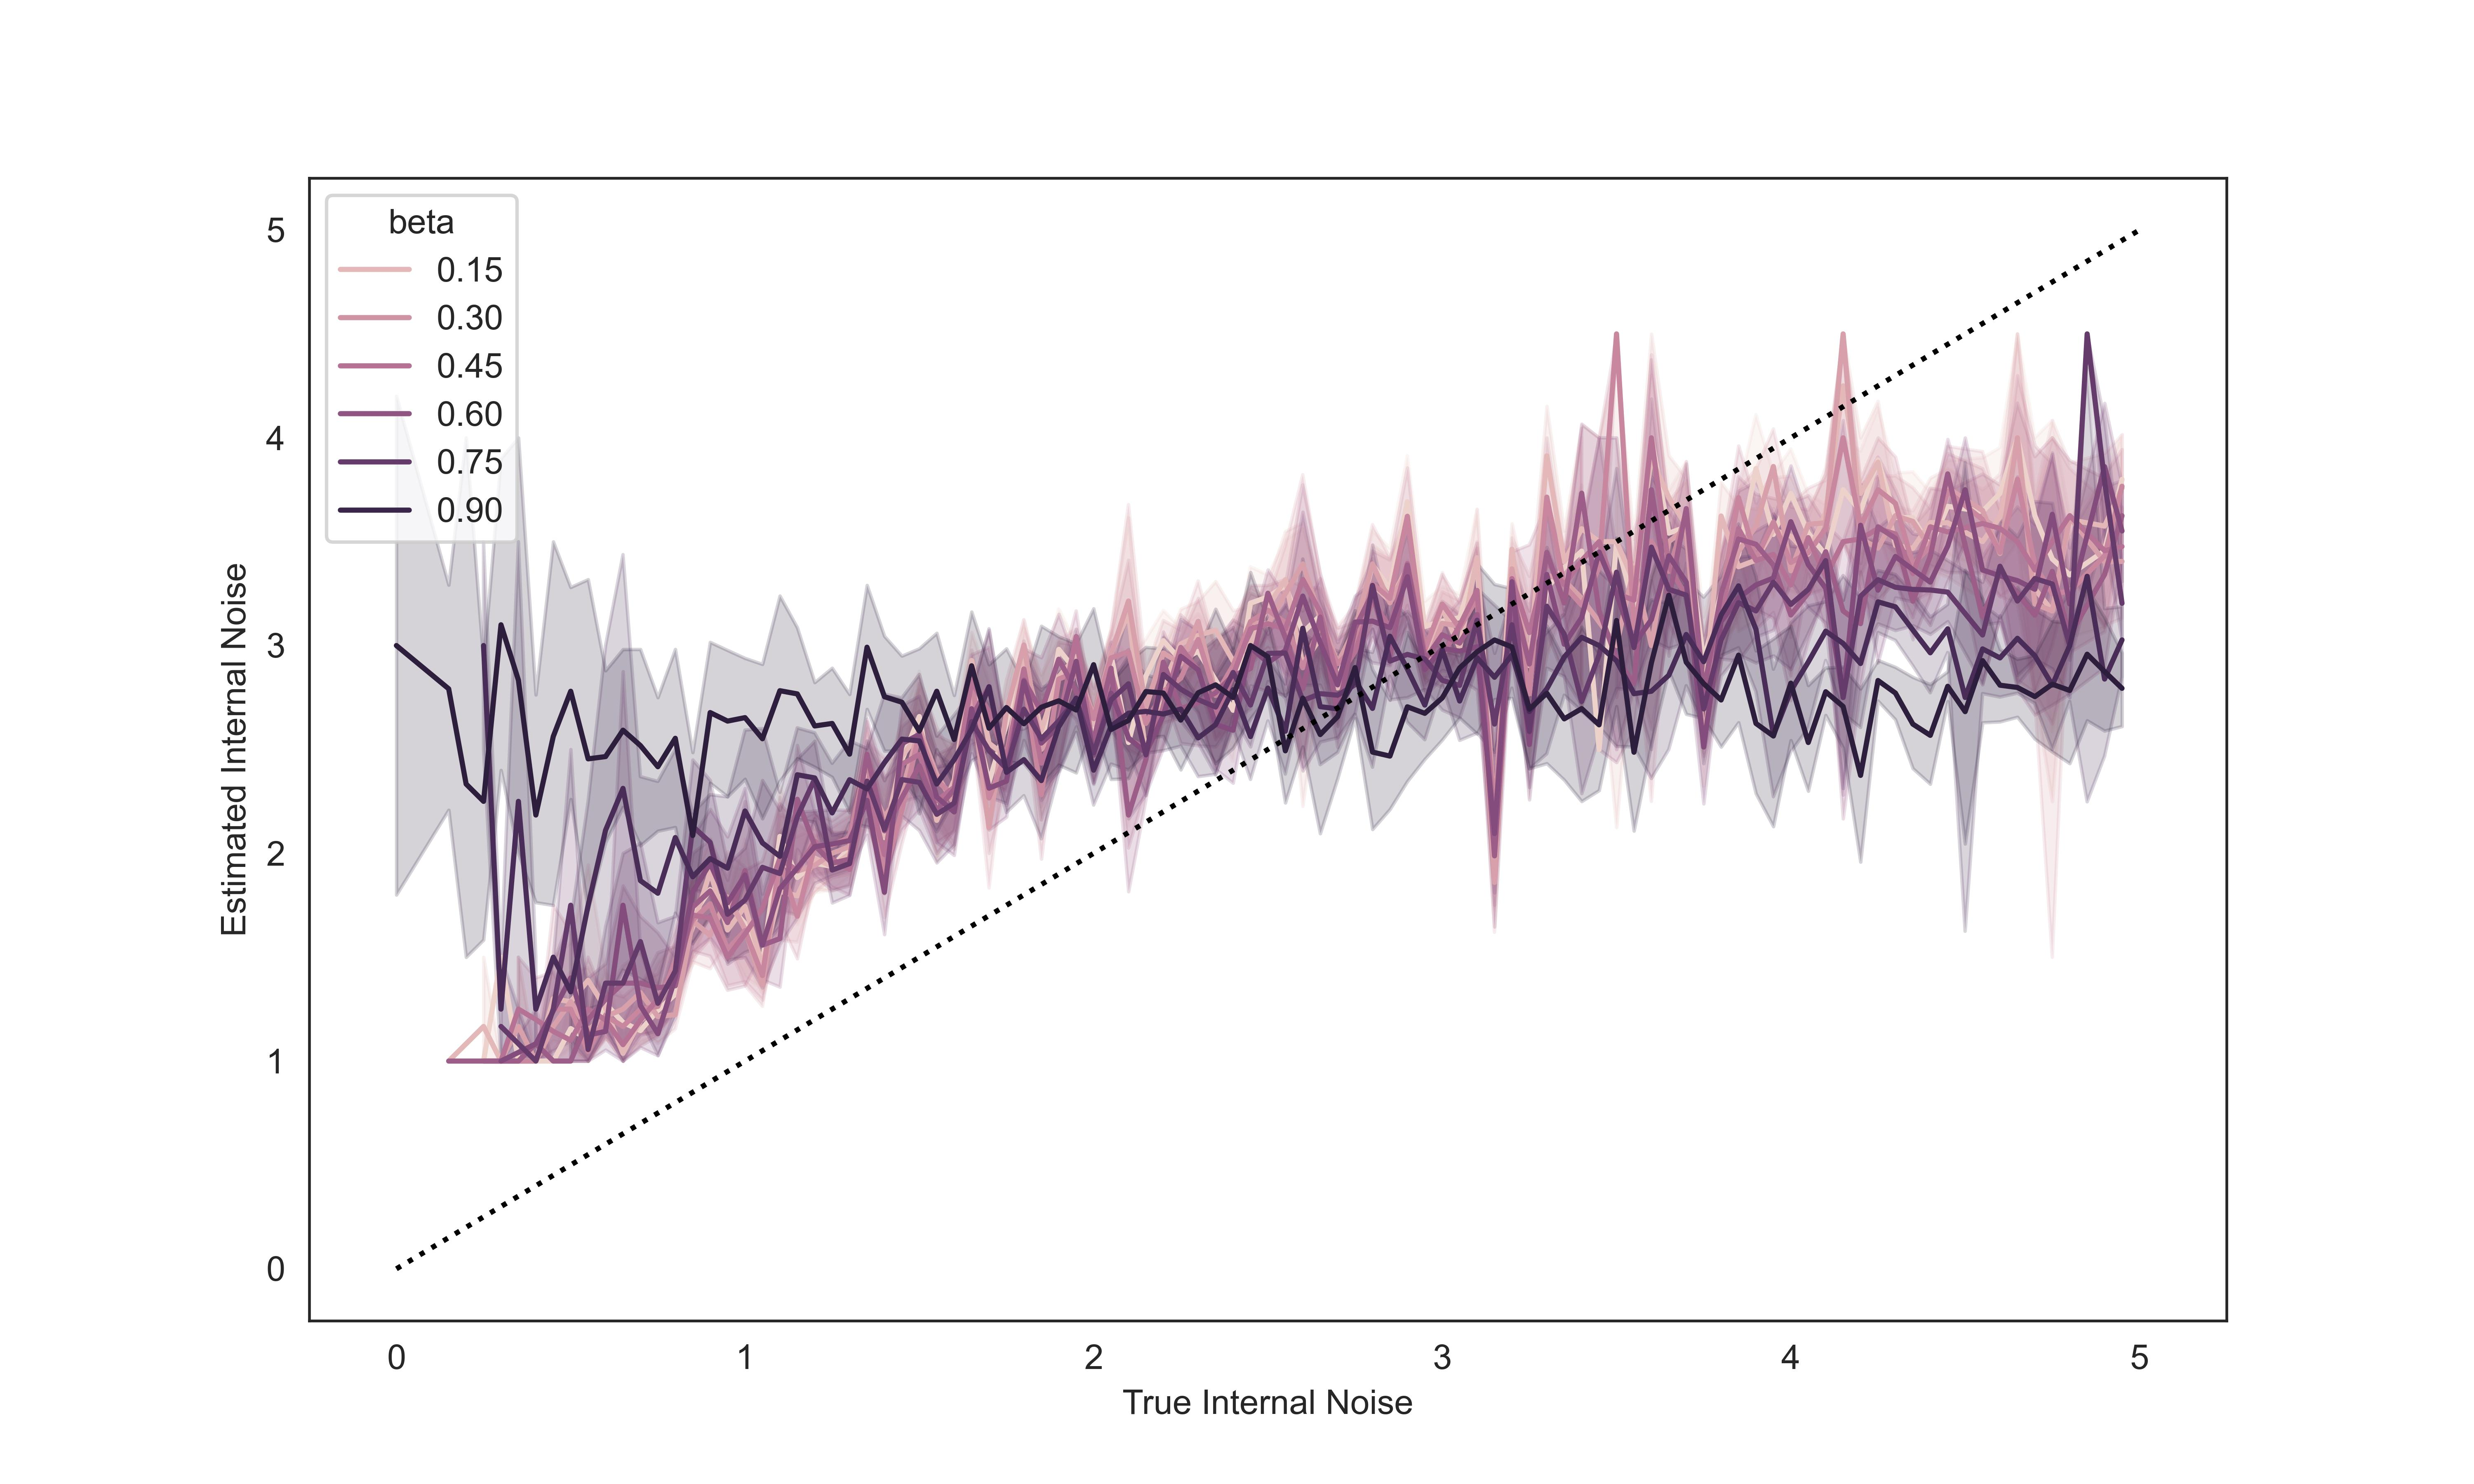
\includegraphics[width=15cm]{MainLayout/Images/chapter5/overestimation_noise.jpg}
    \caption{Main Title for First Image \\ \small Subtitle for the first graphic.}
    \label{fig:overestimation_noise}
\end{figure}


In the double-pass experiment, excessive responses may occur in repeated trials, potentially leading to false probabilities of agreement, making them appear to have low internal noise, despite poor cognitive flexibility. Conversely, if these behaviors do not manifest within the repeated trials, they may go undetected by internal noise estimates, leading to underestimation of internal noise. Additionally, because our kernel estimation relies on the average of responses, some patients may appear to have representations similar to controls, despite underlying perseverative tendencies. This raises the question of whether our regression-based method for classifcation images is truly optimal or if it leads to an over- or underestimation of their deficits.

\begin{figure}[ht!]
    \centering
    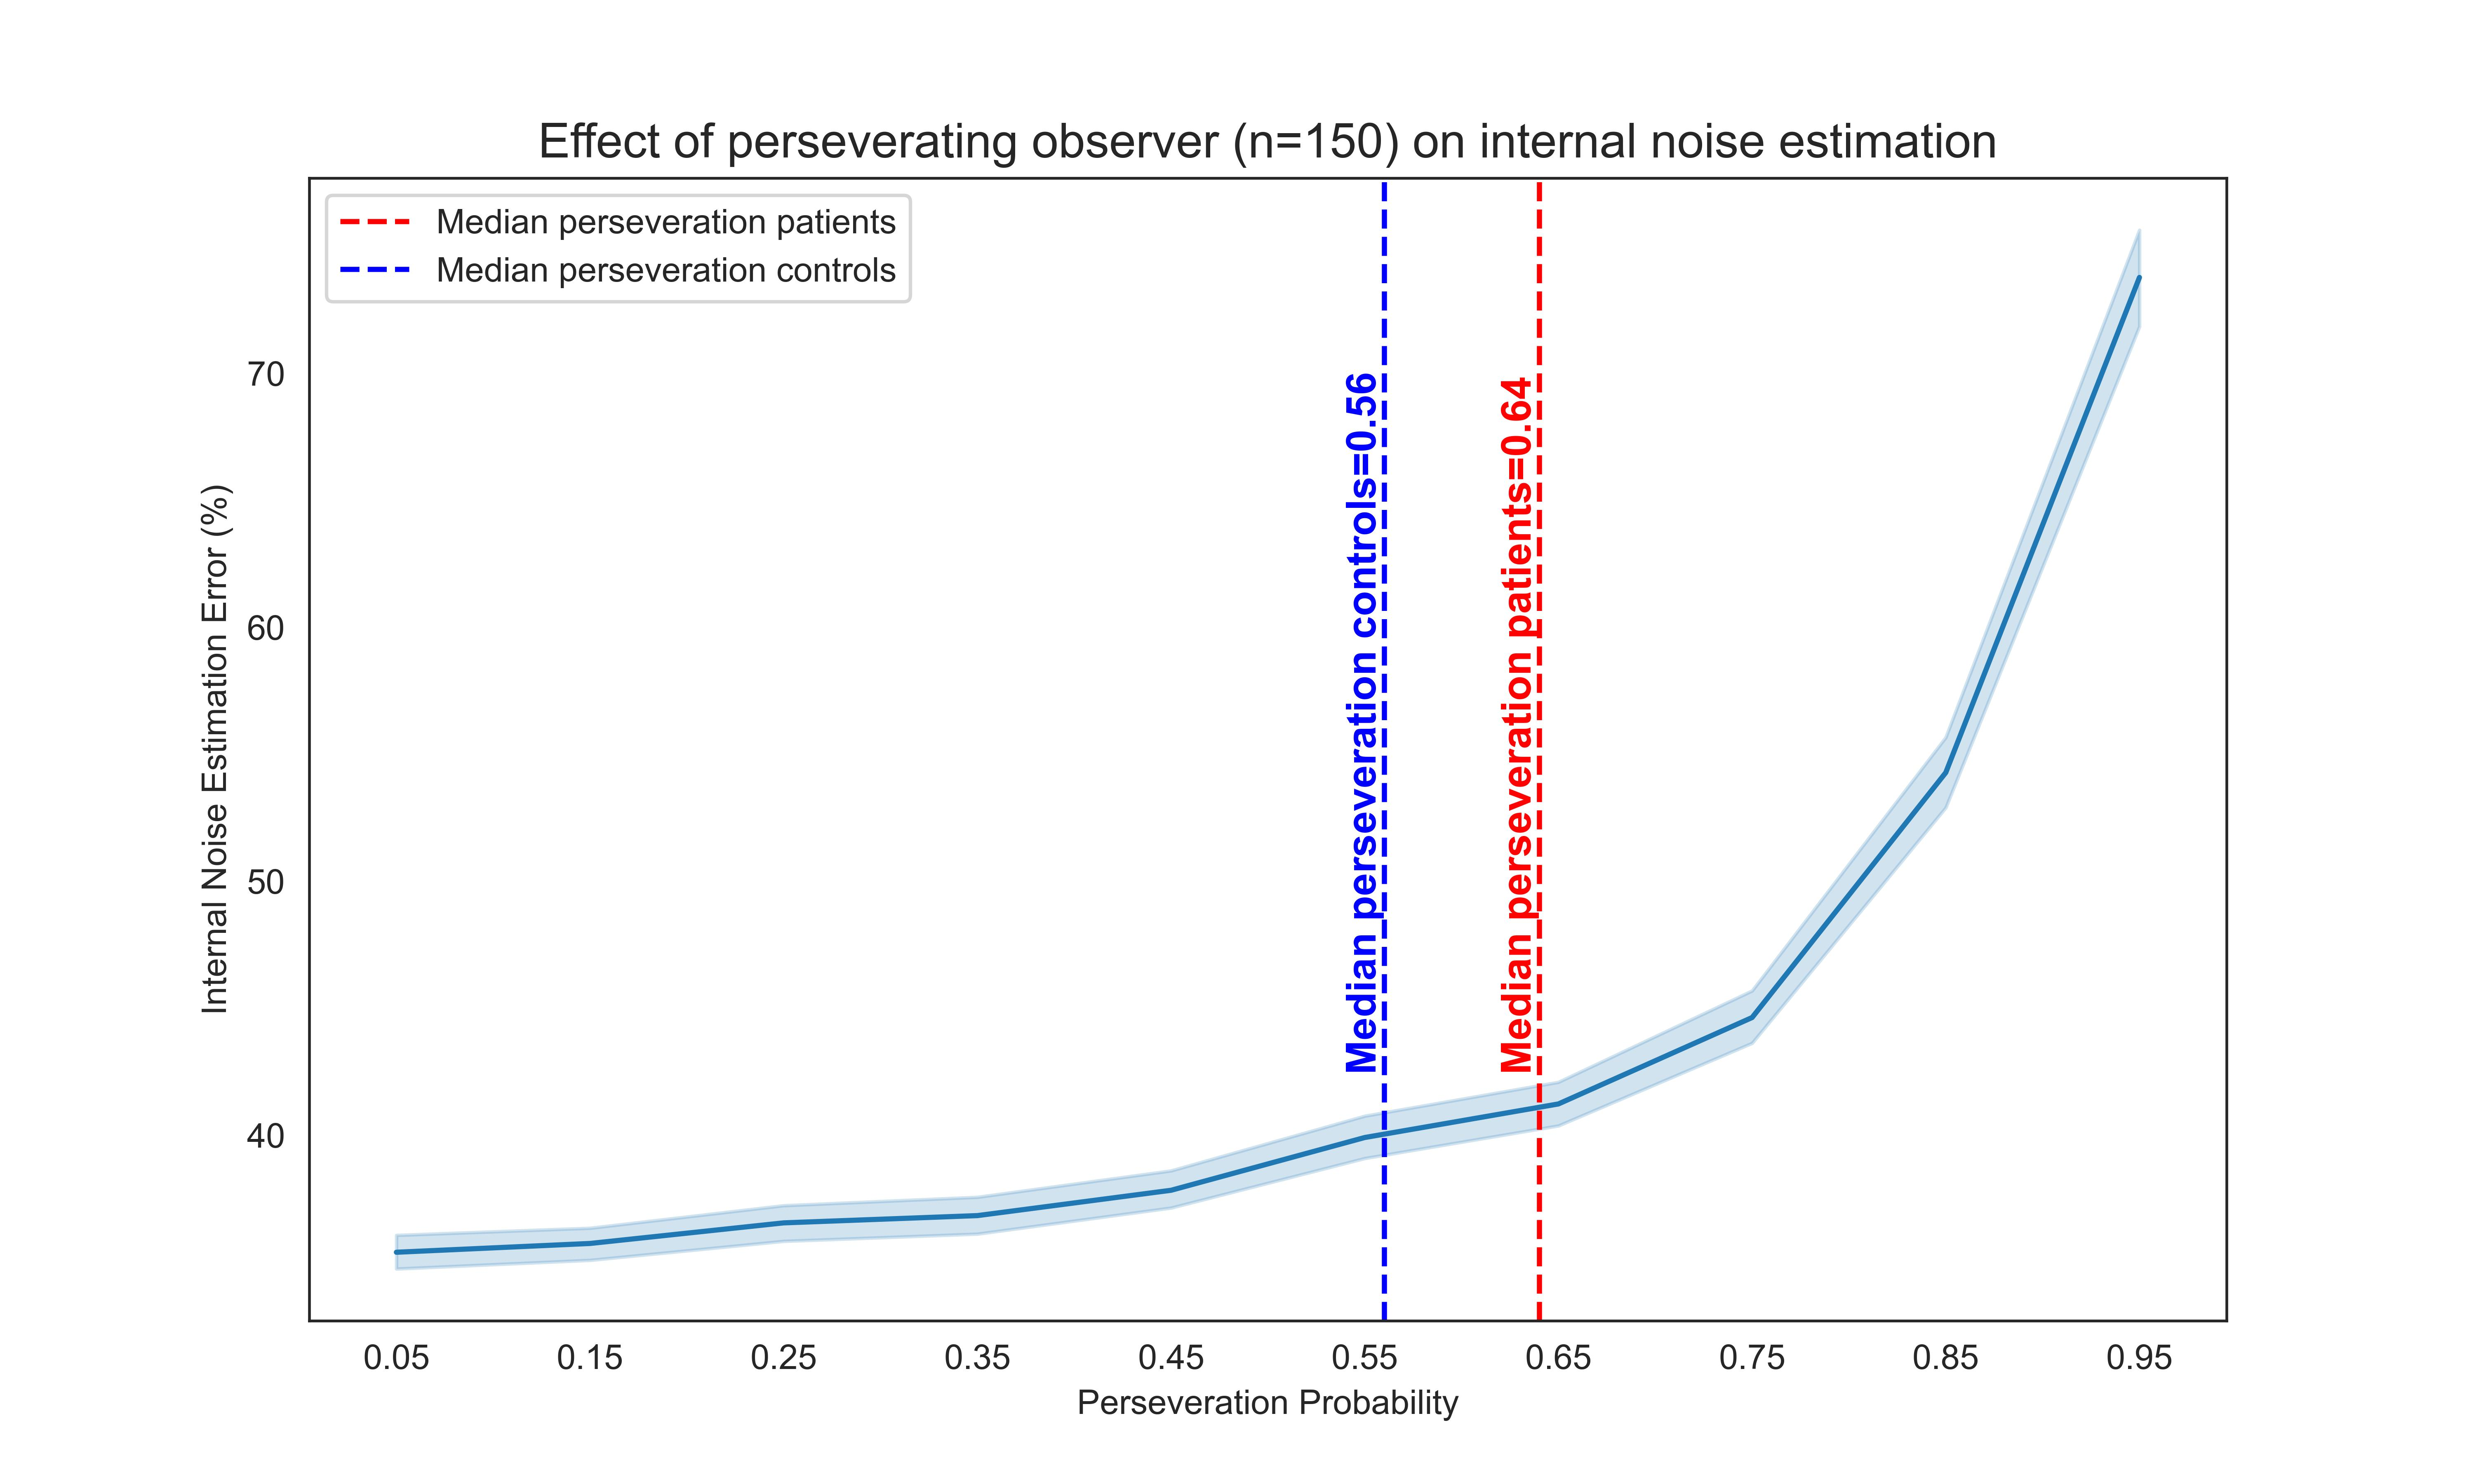
\includegraphics[width=15cm]{MainLayout/Images/chapter5/noise_perseverating_observer.jpg}
    \caption{Main Title for First Image \\ \small Subtitle for the first graphic.}
    \label{fig:noise_perseverating_observer}
\end{figure}



Upper Limit Problem (>5):
Studies (e.g., \cite{neri_how_2010}) suggest that noise estimates beyond IN > 5 should be considered unreliable.
If the estimated internal noise exceeds this range, the model may no longer capture perceptual variability but instead reflect response inconsistencies, such as perseveration, impulsivity, or lapses in attention.
A critical methodological limitation is that for participants exhibiting high internal noise, the estimated percentage of agreement (Pa) may approach chance levels, making it indistinguishable from completely random responses. In such cases, Monte Carlo simulations may fail to differentiate whether a patient genuinely exhibits pathologically high internal noise or if they are simply responding randomly due to task disengagement. The issue is exacerbated by the fact that, unlike low-level perceptual tasks where there is a correct or incorrect response, the present study involves a higher-level prosody classification task in which responses are subjective and based on an individual’s mental representation rather than an objective standard. This makes it even more challenging to attribute response variability solely to internal noise rather than to shifts in perceptual strategies.


\section {Problem statement} 
